% Provenance (never printed): see sources/outline_sources.md (Year 1: grain size and sorting;
% bedforms and sedimentary structures; fluvial, deltaic, shoreline and deep-sea deposits).
% Exercise and problem values in the Book 3 scratch calculator calc/ch21.py; figure data
% from figdata/bachelor-1/grain_size.py. Meander and delta are Book 1's (g5), sediment and
% sedimentary layer Book 1's (g7), beach Book 1's (g9); the loads, settling, the threshold
% of motion and the Hjulstrom diagram are ch. 20's; the vector mean is ch. 6's. Facies
% models and Walther's law belong to the Year 3 volume (prose pointer only). Pelagic
% sediments are ch. 22's.
\chapter{Klastische sedimenten en hun milieus}\label{ch:b1:clastic-sediments}

Neem een handvol zand op een strand en laat het door de vingers lopen: de korrels zijn bijna allemaal even groot, afgerond en schoon, en zij stromen als water. Een paar honderd kilometer landinwaarts, aan de voet van een heuvel die door een oude gletsjer is achtergelaten, is de grond een stijf mengsel van zwerfstenen, kiezels, zand en modder, zonder orde. De twee afzettingen bestaan uit hetzelfde soort puin, afgebroken van dezelfde soorten gesteente; wat ze scheidt, is hoe de korrels reisden en waar zij tot rust kwamen. Een golf die duizenden keren per dag op en neer over een strand loopt, sorteert de korrels naar grootte, voert de fijne weg en rondt de rest af; ijs voert alles mee wat het oppikt en laat het allemaal tegelijk vallen wanneer het smelt. Dit hoofdstuk leert zulke verhalen te lezen uit de korrels zelf, uit de structuren die zij op de bodems van rivieren en zeeën bouwen, en uit de volgorde waarin de afzettingen zijn opgestapeld.

\begin{recall}
Een sediment is los materiaal dat door water, wind of ijs wordt neergelegd, en na verloop van tijd stapelen sedimenten zich op in lagen die verharden tot sedimentair gesteente (Boek~1, klassen~6 en~7). Een rivier die van de ene kant naar de andere over haar uiterwaarde slingert, vormt meanders; waar zij de zee of een meer bereikt en haar vracht laat vallen, bouwt zij een delta; golven stapelen zand op tot stranden en verplaatsen het langs de kust door langsstroming (Boek~1, klassen~5 en~9). Een rivier voert haar vracht als \omterm{def:b1:erosion-transport:load}{bodemvracht}, \omterm{def:b1:erosion-transport:load}{zwevende vracht} en \omterm{def:b1:erosion-transport:load}{opgeloste vracht}; een korrel zinkt met haar \omterm{def:b1:erosion-transport:settling}{bezinksnelheid}; zij begint te bewegen wanneer de \omterm{def:b1:erosion-transport:bed-shear}{bodemschuifspanning} haar \omterm{def:b1:erosion-transport:threshold}{drempel van beweging} overschrijdt, en het \omterm{def:b1:erosion-transport:hjulstrom}{diagram van Hjulström} toont de gemiddelde snelheden van erosie, transport en afzetting tegen de korrelgrootte (\cref{ch:b1:erosion-transport}). Het vectorgemiddelde van een reeks richtingen is de richting van de som van hun eenheidsvectoren (\cref{def:b1:field-lab-methods-1:mean-orientation}).
\end{recall}

\section{Korrelgrootte en sortering}\label{sec:b1:clastic-sediments:grain-size}

De grootte van de korrels is het eerste wat een geoloog in een klastisch sediment noteert, een sediment dat uit fragmenten van oudere gesteenten is opgebouwd, omdat zij de energie meet van de stroming die het heeft neergelegd. Korrelgroottes in de natuur beslaan meer dan zeven ordes van grootte, van zwerfstenen van meters doorsnede tot kleideeltjes van een duizendste millimeter breed, en zij worden op een schaal van verhoudingen gemeten.

\begin{definition}[Korrelgroottenschaal, phi-schaal]\label{def:b1:clastic-sediments:grain-size}
De \emph{korrelgroottenschaal}\index{korrelgroottenschaal} van de sedimentologie verdeelt de diameters van korrels in klassen waarvan de grenzen van de ene klasse naar de volgende verdubbelen, te beginnen bij \qty{1}{mm}; elke klasse heeft een naam (zand, silt\ldots). De \emph{phi-schaal}\index{phi-schaal} drukt een diameter $d$ uit door
\[
  \varphi = -\log_2 \frac{d}{\qty{1}{mm}},
\]
zodat $d = 2^{-\varphi}$~mm: \qty{1}{mm} is $\varphi = 0$, \qty{2}{mm} is $\varphi = -1$, \qty{0.25}{mm} is $\varphi = 2$, en fijnere korrels hebben grotere waarden van $\varphi$.
\end{definition}
% ledger: folk:udden-krumbein, folk:wentworth-classes, usgs:wentworth-phi

Op de \omterm{def:b1:clastic-sediments:grain-size}{phi-schaal} is elke klasse van de \omterm{def:b1:clastic-sediments:grain-size}{korrelgroottenschaal} één eenheid breed: een klasse die van $d$ tot $2d$ loopt, loopt van $\varphi$ tot $\varphi - 1$. De hoofdklassen, met de namen die gewoon in gebruik zijn, staan in \cref{tab:b1:clastic-sediments:classes}.

\begin{table}[htbp]
\centering\small
\begin{tabular}{@{}lll@{}}
\hline
klasse & diameter (\si{mm}) & $\varphi$ \\
\hline
zwerfsteen & boven 256 & onder $-8$ \\
kei & 64 tot 256 & $-6$ tot $-8$ \\
kiezel & 4 tot 64 & $-2$ tot $-6$ \\
granule & 2 tot 4 & $-1$ tot $-2$ \\
zand (zeer grof, grof, middelgrof, fijn, zeer fijn) & $1/16$ tot 2 & 4 tot $-1$ \\
silt (grof, middelgrof, fijn, zeer fijn) & $1/256$ tot $1/16$ & 8 tot 4 \\
klei & onder $1/256$ (\qty{3.9}{\micro m}) & boven 8 \\
\hline
\end{tabular}
\caption{De klassen van korrelgrootte. De vijf klassen van zand zijn elk één phi-eenheid breed, van zeer grof (1 tot \qty{2}{mm}) tot zeer fijn ($1/16$ tot $1/8$~mm), en zo ook de vier klassen van silt. Sommige onderzoekers leggen de ondergrens van silt bij 9 in plaats van $8\,\varphi$. Grind is de algemene naam voor korrels grover dan \qty{2}{mm}, en modder voor het mengsel van silt en klei.}
\label{tab:b1:clastic-sediments:classes}
\end{table}
% ledger: folk:wentworth-classes, usgs:wentworth-phi

Het woord \emph{klei} heeft in dit boek twee betekenissen: hier is het een korrelgroottenklasse, in \cref{ch:b1:weathering-clays} een familie van mineralen. De meeste deeltjes van kleigrootte zijn kleimineralen en de meeste kleimineralen zijn van kleigrootte, maar de twee vallen niet samen: kwarts dat zeer fijn is gemalen is van kleigrootte, en een kaolinietplaatje kan de grootte van silt hebben.

\emph{Het meten van de grootte.} Grind wordt korrel voor korrel met schuifmaat gemeten. Zand wordt gezeefd: een stapel zeven met mazen bij elke gehele of halve phi-eenheid wordt geschud, en het op elke zeef achtergebleven deel wordt gewogen. Silt en klei, fijner dan $4\,\varphi$, worden gemeten door bezinking: het sediment wordt in water geroerd, en omdat elke korrel zinkt met een snelheid die door haar grootte wordt bepaald (wet van Stokes, \cref{prop:b1:erosion-transport:stokes}), vertelt de massa die op een gegeven diepte en tijd nog in suspensie is, hoeveel van het monster fijner is dan een gegeven diameter. Lasersystemen die de verstrooiing van licht door de korrels meten, zijn nu ook gangbaar. Het resultaat is een lijst van het gewichtspercentage in elke klasse.

\begin{definition}[Gemiddelde korrelgrootte, sortering]\label{def:b1:clastic-sediments:sorting}
Laat de korrelgroottes van een sediment, in phi-eenheden, de verdeling hebben die door het gewicht in elke klasse wordt gegeven. Haar \emph{gemiddelde korrelgrootte}\index{gemiddelde korrelgrootte} is het gemiddelde van die verdeling, en haar \emph{sortering}\index{sortering} is de spreiding van de verdeling, gemeten door haar standaardafwijking in phi-eenheden: een sediment is goed gesorteerd wanneer haar korrels bijna allemaal van één grootte zijn, en slecht gesorteerd wanneer zij vele klassen bestrijken. Beide worden berekend hetzij uit de percentages in de klassen, met de methode van de momenten, hetzij uit de cumulatieve kromme, met de grafische maten van Folk:
\[
  M_z = \frac{\varphi_{16} + \varphi_{50} + \varphi_{84}}{3}, \qquad
  \sigma_I = \frac{\varphi_{84} - \varphi_{16}}{4} + \frac{\varphi_{95} - \varphi_{5}}{6.6},
\]
waarbij $\varphi_p$ de grootte in phi-eenheden is waarboven $p$ procent van het monster grover is.
\end{definition}
% ledger: folk:graphic-measures

\begin{method}[Gemiddelde en sortering uit een zeefanalyse]\label{met:b1:clastic-sediments:graphic}
\begin{enumerate}
  \item Noteer het gewichtspercentage $w_i$ in elke klasse, van de grofste tot de fijnste, en controleer dat de som \qty{100}{\percent} is (of deel erdoor).
  \item \emph{Methode van de momenten.} Met $x_i$ het middelpunt van klasse $i$ in phi-eenheden, bereken het gemiddelde $m = \sum w_i x_i / 100$ en de standaardafwijking $s = \sqrt{\sum w_i (x_i - m)^2 / 100}$.
  \item \emph{Grafische maten.} Tel de percentages op om het gewichtspercentage grover dan elke klassegrens te krijgen, en zet het uit tegen $\varphi$: dit is de cumulatieve kromme.
  \item Lees erop af, door lineaire interpolatie tussen klassegrenzen, de groottes $\varphi_5$, $\varphi_{16}$, $\varphi_{50}$, $\varphi_{84}$ en $\varphi_{95}$.
  \item Bereken $M_z$ en $\sigma_I$ (\cref{def:b1:clastic-sediments:sorting}), reken $M_z$ om in millimeter met $d = 2^{-M_z}$, en benoem de \omterm{def:b1:clastic-sediments:sorting}{sortering} aan de hand van de schaal hieronder.
\end{enumerate}
\end{method}

De twee methoden geven bijna dezelfde antwoorden, en de reden is de volgende eigenschap.

\begin{proposition}[Grafische maten van een normale verdeling]\label{prop:b1:clastic-sediments:normal}
Als de groottes van een sediment, in phi-eenheden, normaal verdeeld zijn met gemiddelde $\mu$ en standaardafwijking $\sigma$, dan is $M_z = \mu$ en $\sigma_I = 0.996\,\sigma$.
\end{proposition}

\begin{proof}
Voor een normale verdeling hangt de fractie van de waarden beneden $\mu + z\sigma$ alleen van $z$ af; de fractie beneden $\mu + 0.9945\,\sigma$ is \qty{84}{\percent} en beneden $\mu + 1.6449\,\sigma$ is zij \qty{95}{\percent} (waarden van de normale verdeling, aangenomen). Door symmetrie is $\varphi_{50} = \mu$, $\varphi_{16} = \mu -
0.9945\,\sigma$, $\varphi_{84} = \mu + 0.9945\,\sigma$, $\varphi_5 = \mu -
1.6449\,\sigma$ en $\varphi_{95} = \mu + 1.6449\,\sigma$ (de percentielen tellen het grovere deel, dat wil zeggen de kleinere $\varphi$, maar de verdeling is symmetrisch). Dan is $M_z = (3\mu)/3 = \mu$ en
\[
  \sigma_I = \frac{2 \times 0.9945\,\sigma}{4} + \frac{2 \times 1.6449\,\sigma}{6.6}
  = (0.4972 + 0.4985)\,\sigma = 0.996\,\sigma. \qedhere
\]
\end{proof}

De constante 6.6 in de formule van Folk is hierop gekozen: het interval van het 5e tot het 95e percentiel omvat $3.29$ standaardafwijkingen van een normale verdeling, en de formule middelt de schattingen van $\sigma$ uit de twee intervallen, $(\varphi_{84}-\varphi_{16})/2$ en $(\varphi_{95}-\varphi_5)/3.3$. Door de staarten én de centrale twee derde van de kromme te gebruiken, wordt $\sigma_I$ gevoelig voor de grove en fijne bijmengingen die het meeste vertellen over hoe een sediment is afgezet.

\begin{omfigure}
\begin{tikzpicture}[font=\small]
% grain-size histograms and cumulative curves of two invented samples (figdata/bachelor-1/grain_size.py)
\begin{axis}[name=a, width=7.3cm, height=6cm, xmin=-5.5, xmax=10.5, ymin=0, ymax=90,
    xlabel={korrelgrootte $\varphi$}, ylabel={gewichtspercentage in de klasse},
    title={\footnotesize (a) histogrammen}, xtick={-4,-2,...,10}, ytick={0,20,...,80},
    legend style={at={(0.03,0.97)}, anchor=north west, font=\scriptsize}, legend cell align=left]
  \addplot[ybar interval, fill=omDef!35, draw=omDef, area legend] table[x=phi, y=wt] {figdata/out/bachelor-1-grain_size-step-beach.dat} \closedcycle;
  \addplot[const plot, fill=omThm!20, draw=omThm, fill opacity=0.6, area legend] table[x=phi, y=wt] {figdata/out/bachelor-1-grain_size-step-till.dat} \closedcycle;
  \legend{strandzand (halve-phi-klassen), keileem (hele-phi-klassen)}
\end{axis}
\begin{axis}[at={(a.east)}, anchor=west, xshift=1.6cm, width=7.3cm, height=6cm, xmin=-5.5, xmax=10.5, ymin=0, ymax=100,
    xlabel={korrelgrootte $\varphi$}, ylabel={gewichtspercentage grover},
    title={\footnotesize (b) cumulatieve curven}, xtick={-4,-2,...,10}, ytick={0,16,50,84,100},
    grid=major, grid style={black!10}]
  \addplot[omDef, very thick, mark=*, mark size=1.2pt] table[x=phi, y=cum] {figdata/out/bachelor-1-grain_size-cum-beach.dat};
  \addplot[omThm, very thick, mark=*, mark size=1.2pt] table[x=phi, y=cum] {figdata/out/bachelor-1-grain_size-cum-till.dat};
  \node[font=\footnotesize, omDef, anchor=west] at (axis cs:2.9,40) {strandzand};
  \node[font=\footnotesize, omThm, anchor=west] at (axis cs:5.4,72) {keileem};
\end{axis}
\end{tikzpicture}

{\small De grootteverdelingen van twee sedimenten, uit zeef- en bezinkingsanalyses (verzonnen gegevens). (a)~Gewichtspercentage in elke klasse: het strandzand valt bijna geheel in drie halve-phi-klassen van middelgrof en fijn zand; de morene verspreidt zich over vijftien phi-klassen, van kiezels tot klei. (b)~De cumulatieve krommen, het gewichtspercentage grover dan elke grootte: hoe steiler de kromme, hoe beter de \omterm{def:b1:clastic-sediments:sorting}{sortering}. De grafische maten, afgelezen bij 5, 16, 50, 84 en 95 procent, geven voor het zand $M_z = 2.25\,\varphi$ (\qty{0.21}{mm}) en $\sigma_I =
0.36\,\varphi$, voor de morene $M_z = 1.83\,\varphi$ en $\sigma_I = 3.84\,\varphi$.}
\label{fig:b1:clastic-sediments:grain-size}
\end{omfigure}
% ledger: folk:graphic-measures

\emph{Woorden voor de \omterm{def:b1:clastic-sediments:sorting}{sortering}.} Uit veel gemeten sedimenten stelde Folk een verbale schaal voor $\sigma_I$ voor: onder \num{0.35} zeer goed gesorteerd, \num{0.35} tot \num{0.50} goed gesorteerd, \num{0.50} tot \num{0.71} matig goed gesorteerd, \num{0.71} tot \num{1.0} matig gesorteerd, \num{1.0} tot \num{2.0} slecht gesorteerd, \num{2.0} tot \num{4.0} zeer slecht gesorteerd, en boven \num{4.0} uiterst slecht gesorteerd. De beste \omterm{def:b1:clastic-sediments:sorting}{sortering} die natuurlijke sedimenten bereiken, is ongeveer \num{0.20} tot \num{0.25}, en het zand van \omterm{def:b1:clastic-sediments:bedform}{duinen} en stranden dat hij mat, lag tussen \num{0.25} en \num{0.35}; rivierafzettingen liepen van \num{0.40} tot \num{2.5}, de silt en klei van uiterwaarden en continentale platen van ongeveer \num{2.0} tot \num{3.5}, en het slechtst gesorteerd van alles waren glaciale morenen en modderstromen. Het strandzand van de figuur, op \num{0.36}, is goed gesorteerd, aan de rand van zeer goed gesorteerd; de morene, op \num{3.84}, zeer slecht gesorteerd. In de morene geeft de methode van de momenten een gemiddelde van $1.89\,\varphi$ en een standaardafwijking van $3.64\,\varphi$, dicht bij de grafische waarden; de verschillen komen van de staarten en de asymmetrie van de verdeling.
% ledger: folk:sorting-classes, folk:natural-sorting

De \omterm{def:b1:clastic-sediments:sorting}{sortering} is een verslag van het transport. Een stroming sorteert haar vracht omdat de korrels die zij kan verplaatsen en in suspensie houden, van hun grootte afhangen (\cref{sec:b1:erosion-transport:threshold}): golven op een strand en wind over een \omterm{def:b1:clastic-sediments:bedform}{duin} bewerken dezelfde korrels steeds opnieuw, verwijderen de fijnere en laten die te zwaar om te bewegen achter, en hun afzettingen zijn de best gesorteerde van alle. IJs, puinstromen en de plotselinge lozing van een vloed sorteren niets.

\emph{Vorm en afrondingsgraad.} De afrondingsgraad van een korrel beschrijft de scherpte van haar hoeken, los van haar algemene vorm: Wadell definieerde haar als het gemiddelde krommingsradius van de hoeken gedeeld door de straal van de grootste cirkel die in de omtrek van de korrel past, van 1 voor een bol tot bijna 0 voor een splinter. Meten is tijdrovend, en korrels worden daarom vergeleken met tabellen van foto's; op de schaal van Wadell hebben de meeste zandkorrels afrondingsgraden van \num{0.3} tot \num{0.4}, en op de logaritmische schaal van Folk, van 0 (zeer hoekig) tot 6 (zeer rond), ongeveer \num{2.5}, subhoekig. Afronding gaat langzaam voor zand: door wind verplaatst kwarts rondt veel sneller af dan kwarts dat door water wordt meegevoerd, dat de botsingen dempt, en strandzand sneller dan rivierzand, terwijl zandkorrels in rivieren nauwelijks worden afgerond. Kiezels worden snel afgerond in rivieren, de zachte eerst: in de Colorado bereiken kalksteenkiezels binnen enkele mijlen hun eindafronding, terwijl kwartskiezels ongeveer 150 mijl nodig hebben om hen in te halen.
% ledger: folk:roundness, folk:rounding

\begin{definition}[Textuurrijpheid, samenstellingsrijpheid]\label{def:b1:clastic-sediments:maturity}
De \emph{textuurrijpheid}\index{textuurrijpheid} van een zand of zandsteen meet hoe ver de \omterm{def:b1:clastic-sediments:sorting}{sortering}, schuring en uitzeving van de stroming er aan hebben gewerkt, in vier trappen: \emph{onrijp}, met meer dan \qty{5}{\percent} kleimatrix; \emph{subrijp}, met minder klei maar slecht gesorteerde korrels ($\sigma > 0.5\,\varphi$); \emph{rijp}, met weinig of geen klei en goed gesorteerd ($\sigma < 0.5\,\varphi$) maar hoekige korrels; \emph{superrijp}, zonder klei en met korrels die zowel goed gesorteerd als goed afgerond zijn. Haar \emph{samenstellingsrijpheid}\index{samenstellingsrijpheid} meet hoe ver de onstabiele mineralen en gesteentefragmenten zijn verwijderd, zodat kwarts overblijft: zij is hoog in een zandsteen van bijna zuiver kwarts en laag in een zandsteen die rijk is aan \omterm{def:b1:rock-forming-minerals:groups}{veldspaat}, \omterm{def:b1:rock-forming-minerals:groups}{mica} of gesteentefragmenten.
\end{definition}
% ledger: folk:maturity, folk:mineral-maturity

De \omterm{def:b1:clastic-sediments:maturity}{textuurrijpheid} wordt uit de afzetting gelezen zoals zij is neergelegd: kleimineralen die later in de poriën kristalliseerden, en de cementen die de korrels binden (\cref{ch:b1:diagenesis-basins}), tellen niet mee. Zij weerspiegelt de energie van de plaats van afzetting: onrijpe sedimenten hopen zich op in uiterwaarden, aanspoelwaaiers en lagunes, waar stromingen zwak zijn of de afzetting te snel is voor de korrels om bewerkt te worden, en superrijpe op stranden en in woestijnduinen, waar energie zonder einde op de korrels wordt besteed. De \omterm{def:b1:clastic-sediments:maturity}{samenstellingsrijpheid} volgt uit schuring en verwering samen. \omterm{def:b1:rock-forming-minerals:groups}{Veldspaat}, zachter dan kwarts en met een goede splijting, wordt sneller afgesleten; een arkose van hoekig kwarts en \omterm{def:b1:rock-forming-minerals:groups}{veldspaat} van dezelfde grootte kan door schuring alleen eindigen als een superrijpe zandsteen waarin het zand bijna helemaal uit kwarts bestaat en het \omterm{def:b1:rock-forming-minerals:groups}{veldspaat} alleen als silt overleeft. Verwering, in het brongebied en tijdens lange opslag onderweg, doet hetzelfde door veldspaten in klei om te zetten (\cref{sec:b1:weathering-clays:hydrolysis}). Zandsteen die in tijden van korstelijke onrust is afgezet, snel geërodeerd uit rijzende bergen, is vaak onrijp in beide opzichten; die uit rustige tijden, lang opnieuw bewerkt, zijn meestal superrijpe kwartszandstenen; maar uitzonderingen zijn talrijk, en elke samenstelling kan in elke trap van \omterm{def:b1:clastic-sediments:maturity}{textuurrijpheid} voorkomen.
% ledger: folk:maturity, folk:mineral-maturity

\section{Bodemvormen en sedimentaire structuren}\label{sec:b1:clastic-sediments:bedforms}

Wanneer een stroming zand over een bodem beweegt, blijft de bodem zelden vlak: zij organiseert zich in golven van zand die met de stroming meereizen. Deze vormen, en de laagdeling die zij binnen de afzetting achterlaten, zijn het meest rechtstreekse verslag van de stromingen uit het verleden.

\begin{definition}[Bodemvorm, rimpel, duin]\label{def:b1:clastic-sediments:bedform}
Een \emph{bodemvorm}\index{bodemvorm} is een regelmatig reliëf dat door een stroming op een bodem van losse korrels wordt gevormd, herhaald langs de stroming. Een \emph{rimpel}\index{rimpel} is een kleine bodemvorm, enkele centimeters hoog en 10 tot \qty{20}{cm} van kam tot kam, met een zachte stroomopwaartse (stoss-)zijde en een steile stroomafwaartse (lee-)zijde; een \emph{duin}\index{duin} heeft een soortgelijke vorm maar is minstens tien keer groter, van decimeters tot meters hoog onder water.
\end{definition}
% ledger: southard:ripples-dunes

De stoss-zijde van een \omterm{def:b1:clastic-sediments:bedform}{rimpel} helt onder minder dan ongeveer \ang{10}; haar lee-zijde, het glijvlak, staat bijna onder de rusthoek van zand in water, ongeveer \ang{30}. Zand wordt van de stoss-zijde geërodeerd, over de kam gedragen, en
stort naar beneden of regent op het glijvlak, zodat de hele \omterm{def:b1:clastic-sediments:bedform}{rimpel} stroomafwaarts beweegt, veel langzamer dan het water, door korrels van haar achterkant te nemen en aan haar voorkant toe te voegen. Wind bouwt op het land \omterm{def:b1:clastic-sediments:bedform}{rimpels} en \omterm{def:b1:clastic-sediments:bedform}{duinen} van dezelfde soort, de \omterm{def:b1:clastic-sediments:bedform}{duinen} van woestijnen veel groter dan die van rivieren.
% ledger: southard:ripples-dunes, southard:climb

\begin{proposition}[Migratie van bodemvormen en bodemvracht]\label{prop:b1:clastic-sediments:migration}
Een reeks \omterm{def:b1:clastic-sediments:bedform}{bodemvormen} met driehoekig profiel, van hoogte $H$, die stroomafwaarts beweegt met de snelheid $c$ zonder van vorm te veranderen, door erosie van de stoss-zijden en afzetting op de lee-zijden, voert over de kammen het volume \omterm{def:b1:erosion-transport:load}{bodemvracht} per eenheid breedte en tijd
\[
  q_b = (1 - p)\,\frac{c\,H}{2},
\]
als vaste korrels geteld, waarbij $p$ de porositeit van het zand is.
\end{proposition}

\begin{proof}
Volg de bodem op een vast punt terwijl één \omterm{def:b1:clastic-sediments:bedform}{bodemvorm} passeert, in de tijd $L/c$, $L$ is de lengte ervan. Elke korrel van de \omterm{def:b1:clastic-sediments:bedform}{bodemvorm} boven de lijn van de dalen is over de kam van de \omterm{def:b1:clastic-sediments:bedform}{bodemvorm} erachter gegaan, omdat de \omterm{def:b1:clastic-sediments:bedform}{bodemvorm} alleen beweegt door overdracht van korrels van stoss naar lee. De \omterm{def:b1:clastic-sediments:bedform}{bodemvorm} heeft de dwarsdoorsnede $LH/2$, een driehoek met basis $L$ en hoogte $H$, waarvan het deel $1 - p$ korrels is. Dat volume korrels gaat in de tijd $L/c$ over elke kam, dus de flux is $(1-p)(LH/2)/(L/c) = (1-p)cH/2$. Het deel van de vracht dat over de \omterm{def:b1:clastic-sediments:bedform}{bodemvormen} reist zonder aan de lee-zijde te bezinken, wordt niet geteld, zodat de formule een ondergrens van de \omterm{def:b1:erosion-transport:load}{bodemvracht} geeft.
\end{proof}

\emph{De volgorde van de bodemfasen.} In een laboratoriumgoot met een bodem van middelgrof zand bouwt een toenemende stroming een vaste opeenvolging van bodemconfiguraties op. Onder de \omterm{def:b1:erosion-transport:threshold}{drempel van beweging} blijft de bodem vlak. Net erboven verschijnen \omterm{def:b1:clastic-sediments:bedform}{rimpels}, die bij toenemende stroming worden vervangen door \omterm{def:b1:clastic-sediments:bedform}{duinen}, bij een snelheid van een gematigde fractie van een meter per seconde en binnen enkele centimeters per seconde. Nog sneller vlakken de \omterm{def:b1:clastic-sediments:bedform}{duinen} af, en wordt de bodem weer een vlak, de bovenste vlakke bodem, waarover het zand in een dichte laag en in suspensie beweegt. Ten slotte, wanneer de gemiddelde snelheid $U$ de snelheid $\sqrt{gh}$ van oppervlaktegolven in water van diepte $h$ nadert, dat wil zeggen wanneer het Froude-getal $U/\sqrt{gh}$ naar 1 nadert, vormen het wateroppervlak en de bodem golven in fase, die groeien, steiler worden, breken en opnieuw vormen: antiduinen, genoemd door G.~K. Gilbert in zijn goot-experimenten van 1914, omdat hun kammen stroomopwaarts bewegen. Antiduinen hebben ondiepe, snelle stromingen nodig en zijn onbelangrijk in stromingen die dieper zijn dan enkele meters.
% ledger: southard:ripples-dunes

De korrelgrootte verandert de volgorde. \omterm{def:b1:clastic-sediments:bedform}{Rimpels} vormen zich alleen in zand fijner dan ongeveer \qty{0.8}{mm}; in grof zand en grind gaat de bodem van een vlakke bodem zonder beweging naar een lage vlakke bodem met bewegende korrels en dan rechtstreeks naar \omterm{def:b1:clastic-sediments:bedform}{duinen}. In fijn zand, beneden ongeveer \qty{0.2}{mm}, vormen de \omterm{def:b1:clastic-sediments:bedform}{duinen} zich nooit, en maken de \omterm{def:b1:clastic-sediments:bedform}{rimpels} direct plaats voor de bovenste vlakke bodem. De velden van de bodemfasen worden afgebeeld op diagrammen van snelheid tegen korrelgrootte, getekend voor een gegeven stromingsdiepte.
% ledger: southard:phase-diagram

\begin{omfigure}
\begin{tikzpicture}[font=\footnotesize, >={Stealth[length=4pt]}]
% (a) bed phases with increasing flow (schematic); (b) bed-phase diagram after Southard (schematic)
\begin{scope}
  \foreach \y/\lab in {0/{vlakke bodem,\\ geen beweging}, 1.25/rimpels, 2.5/duinen, 3.75/bovenste bodem, 5.0/antiduinen} {
    \node[anchor=east, align=right] at (-0.15,\y+0.25) {\lab};
  }
  \foreach \y in {0, 1.25, 2.5, 3.75} {\draw[omDef!70!black] (0,\y+0.85) -- (5.5,\y+0.85);}
  % plane bed
  \fill[brown!45] (0,0) rectangle (5.5,0.3);
  % ripples: small, asymmetric (lee side downstream, to the right)
  \fill[brown!45] (0,1.25) -- (0,1.55) \foreach \i in {0,...,10} {-- (\i*0.5+0.4,1.7) -- (\i*0.5+0.5,1.55)} -- (5.5,1.25) -- cycle;
  \draw[brown!70!black] (0,1.55) \foreach \i in {0,...,10} {-- (\i*0.5+0.4,1.7) -- (\i*0.5+0.5,1.55)};
  % dunes: larger asymmetric
  \fill[brown!45] (0,2.5) rectangle (5.5,2.65);
  \fill[brown!45] (0,2.65) -- (1.6,3.05) -- (1.85,2.65) -- (3.45,3.05) -- (3.7,2.65) -- (5.3,3.05) -- (5.5,2.75) -- (5.5,2.65) -- cycle;
  \draw[brown!70!black] (0,2.65) -- (1.6,3.05) -- (1.85,2.65) -- (3.45,3.05) -- (3.7,2.65) -- (5.3,3.05) -- (5.5,2.75);
  % upper plane bed with sheet flow
  \fill[brown!45] (0,3.75) rectangle (5.5,4.05);
  \foreach \x in {0.2,0.6,...,5.4} {\fill[brown!70!black] (\x,4.12) circle[radius=0.025];}
  % antidunes: symmetric waves in phase with the surface
  \fill[brown!45] (0,5.0) -- plot[domain=0:5.5, samples=60] (\x,{5.25+0.08*sin(\x*130)}) -- (5.5,5.0) -- cycle;
  \draw[brown!70!black] plot[domain=0:5.5, samples=60] (\x,{5.25+0.08*sin(\x*130)});
  \draw[omDef!70!black, thick] plot[domain=0:5.5, samples=60] (\x,{5.85+0.12*sin(\x*130)});
  \draw[->, thick] (5.9,0.3) -- node[above, rotate=90, font=\scriptsize] {toenemende stroomsnelheid} (5.9,5.6);
  \draw[->, black!70] (1.5,6.35) -- node[above] {stroming} (4.0,6.35);
  \node[font=\footnotesize] at (2.75,-1.15) {(a) bodemfasen, middelgrof zand};
\end{scope}
% (b) phase diagram (schematic)
\begin{scope}[xshift=7.1cm]
  \draw[->] (0,0) -- (6.2,0);
  \draw[->] (0,0) -- (0,6.2) node[above, align=center] {gemiddelde stroom-\\ snelheid};
  % x positions: x = 2*log10(d/0.06) ; 0.1 mm -> 0.44, 0.2 -> 1.05, 0.8 -> 2.25, 2 -> 3.05, 10 -> 4.44
  \foreach \d/\x in {0.1/0.44, 0.2/1.05, 0.8/2.25, 2/3.05, 10/4.44} {\draw (\x,0) -- (\x,-0.08) node[below] {\d};}
  \node[below] at (5.7,-0.08) {mm};
  \node[anchor=north, font=\scriptsize] at (3.0,-0.5) {korrelgrootte (log)};
  % threshold of motion
  \draw[thick, omThm] (0,1.0) .. controls (1.0,0.85) and (2.0,1.0) .. (3.0,1.5) .. controls (4.0,2.0) .. (6.0,2.9);
  % ripple field upper boundary
  \draw[thick] (0,3.6) .. controls (0.6,3.3) and (0.9,2.6) .. (1.05,2.35);
  \draw[thick] (1.05,2.35) .. controls (1.6,1.9) and (2.0,1.4) .. (2.25,1.15);
  % dune field lower boundary to the right of 0.8 mm
  \draw[thick] (2.25,1.15) .. controls (3.0,1.9) and (4.5,2.9) .. (6.0,3.7);
  % dune upper boundary (to upper plane bed)
  \draw[thick] (1.05,2.35) .. controls (1.5,3.6) and (3.0,4.6) .. (6.0,5.4);
  % antidune boundary
  \draw[thick, dashed] (0,4.9) .. controls (1.0,4.9) and (2.5,5.4) .. (4.0,5.9);
  \node at (0.55,1.9) {rimpels};
  \node at (3.3,3.0) {duinen};
  \node at (4.75,2.5) [rotate=22, font=\scriptsize] {lage vlakke bodem};
  \node at (2.1,0.45) [align=center] {geen beweging};
  \node at (1.45,4.3) {bovenste vlakke bodem};
  \node at (1.3,5.45) {antiduinen};
  \fill (1.05,2.35) circle[radius=1.4pt]; \fill (2.25,1.15) circle[radius=1.4pt];
  \node[font=\footnotesize] at (3.0,-1.15) {(b) bodemfasen, waterdiepte enkele dm};
\end{scope}
\end{tikzpicture}

{\small (a)~De opeenvolging van bodem\-configuraties in middelgrof zand naarmate de stroming versterkt, van onder naar boven, met het water\-oppervlak erboven (schematisch, hoogten overdreven). \omterm{def:b1:clastic-sediments:bedform}{Rimpels} en \omterm{def:b1:clastic-sediments:bedform}{duinen} bewegen stroomafwaarts, antiduinen stroomopwaarts, hun oppervlaktegolven in fase met de bodem. (b)~De velden waarin elke bodemfase stabiel is, tegen de korrelgrootte en de stroomsnelheid, voor een stroming van enkele decimeter diep (schematisch, naar de goot-compilaties van Southard; de doorgetrokken kromme onderaan is de \omterm{def:b1:erosion-transport:threshold}{drempel van beweging}). De twee stippen zijn de drievoudige punten bij ongeveer \qty{0.2}{mm} en \qty{0.8}{mm}: \omterm{def:b1:clastic-sediments:bedform}{rimpels} vormen zich alleen in fijner zand, \omterm{def:b1:clastic-sediments:bedform}{duinen} alleen in grover.}
\label{fig:b1:clastic-sediments:bed-phases}
\end{omfigure}
% ledger: southard:ripples-dunes, southard:phase-diagram

\begin{definition}[Kruislagen, paleostroom]\label{def:b1:clastic-sediments:cross-bedding}
\emph{Kruislagen}\index{kruislagen} is een laagdeling die schuin staat ten opzichte van de hoofdlaagdeling, gemaakt van de opeenvolgende lee-vlakken (voorlagen) van migrerende \omterm{def:b1:clastic-sediments:bedform}{rimpels} of \omterm{def:b1:clastic-sediments:bedform}{duinen}, in eenheden, de sets, begrensd door erosievlakken; kruislagen die door \omterm{def:b1:clastic-sediments:bedform}{rimpels} zijn gemaakt, in sets van enkele centimeters dik, heten kruislaminatie. Een \emph{paleostroom}\index{paleostroom} is de richting van een oude stroming, afgeleid uit de structuren die zij heeft achtergelaten: de voorlagen helen stroomafwaarts, dus is de helling van de kruislagen, zodra de laagdeling weer horizontaal is gemaakt, de richting waarheen de stroming stroomde.
\end{definition}

\begin{proposition}[Klimmende bodemvormen]\label{prop:b1:clastic-sediments:climb}
Een reeks identieke \omterm{def:b1:clastic-sediments:bedform}{bodemvormen}, op afstand $L$, die stroomafwaarts beweegt met de snelheid $c$ terwijl de bodem door afzetting met de snelheid $a$ wordt verhoogd, klimt langs banen die met de bodem de hoek $\theta$ maken, met
\[
  \tan\theta = \frac{a}{c}.
\]
De afzetting is dan een stapel kruislagsets van dikte, gemeten loodrecht op de setgrenzen,
\[
  T = L\,\sin\theta .
\]
Als $a = 0$, blijft niets van de voorlagen behouden.
\end{proposition}

\begin{proof}
Elk punt van een \omterm{def:b1:clastic-sediments:bedform}{bodemvorm}, en in het bijzonder haar dal, beweegt stroomafwaarts over $c\,\mathrm dt$ en omhoog over $a\,\mathrm dt$ in de tijd $\mathrm dt$: het legt een rechte lijn af met helling $a/c$, onder de hoek $\theta$. Het dal van een \omterm{def:b1:clastic-sediments:bedform}{bodemvorm} schuurt alles weg dat onder haar baan en boven de baan van het voorgaande dal ligt, dus zijn de setgrenzen de banen van de dalen: evenwijdige lijnen onder $\theta$, die door punten op afstand $L$ langs de bodem gaan. Twee evenwijdige lijnen onder de hoek $\theta$ met een horizontale lijn, die deze snijden in punten op afstand $L$ van elkaar, liggen op de loodrechte afstand $L\sin\theta$ uiteen. Als $a = 0$ vallen de banen samen met de bodem, is $T = 0$, en wist elk dal de voorlagen die de \omterm{def:b1:clastic-sediments:bedform}{bodemvorm} ervoor had gelegd.
\end{proof}
% ledger: southard:climb

De klimhoek is klein voor de meeste \omterm{def:b1:clastic-sediments:bedform}{duinen} en \omterm{def:b1:clastic-sediments:bedform}{rimpels}, waardoor een set alleen het onderste deel van de voorlagen bewaart, boven afgesneden door het volgende erosievlak: de afgesneden toppen en de tangentiële, buigende basis van \omterm{def:b1:clastic-sediments:cross-bedding}{kruislagen} vertellen welke kant boven was, een van de criteria om te bepalen of een reeks lagen rechtop of omgekeerd staat (\cref{ch:b1:faults-folds-fabrics}). Waar zand snel uit suspensie neerregent, zoals in een afnemende vloed, wordt de klimhoek steil en blijven hele rimpelprofielen behouden, gestapeld als klimmende \omterm{def:b1:clastic-sediments:bedform}{rimpels}.
% ledger: southard:climb

\begin{omfigure}
\begin{tikzpicture}[font=\footnotesize, >={Stealth[length=4pt]}]
% climbing ripples: geometry of the proposition (schematic, theta exaggerated)
% generated by a scratch script: L = 2.4, theta = 12 deg, H = 0.42, lee 39 deg (exaggerated)
\begin{scope}
\clip (0,-0.05) rectangle (7.40,3);
\clip (-1.367,0) -- (-1.367,1.750) -- (0.505,2.170) -- (1.033,1.750) -- (2.905,2.170) -- (3.433,1.750) -- (5.305,2.170) -- (5.833,1.750) -- (7.705,2.170) -- (8.233,1.750) -- (8.233,0) -- cycle;
\fill[brown!12] (-3,0) rectangle (10,3);
\draw[brown!65!black, thin] (-4.000,2.270) -- ++(3.130,-2.490);
\draw[brown!65!black, thin] (-3.800,2.270) -- ++(3.130,-2.490);
\draw[brown!65!black, thin] (-3.600,2.270) -- ++(3.130,-2.490);
\draw[brown!65!black, thin] (-3.400,2.270) -- ++(3.130,-2.490);
\draw[brown!65!black, thin] (-3.200,2.270) -- ++(3.130,-2.490);
\draw[brown!65!black, thin] (-3.000,2.270) -- ++(3.130,-2.490);
\draw[brown!65!black, thin] (-2.800,2.270) -- ++(3.130,-2.490);
\draw[brown!65!black, thin] (-2.600,2.270) -- ++(3.130,-2.490);
\draw[brown!65!black, thin] (-2.400,2.270) -- ++(3.130,-2.490);
\draw[brown!65!black, thin] (-2.200,2.270) -- ++(3.130,-2.490);
\draw[brown!65!black, thin] (-2.000,2.270) -- ++(3.130,-2.490);
\draw[brown!65!black, thin] (-1.800,2.270) -- ++(3.130,-2.490);
\draw[brown!65!black, thin] (-1.600,2.270) -- ++(3.130,-2.490);
\draw[brown!65!black, thin] (-1.400,2.270) -- ++(3.130,-2.490);
\draw[brown!65!black, thin] (-1.200,2.270) -- ++(3.130,-2.490);
\draw[brown!65!black, thin] (-1.000,2.270) -- ++(3.130,-2.490);
\draw[brown!65!black, thin] (-0.800,2.270) -- ++(3.130,-2.490);
\draw[brown!65!black, thin] (-0.600,2.270) -- ++(3.130,-2.490);
\draw[brown!65!black, thin] (-0.400,2.270) -- ++(3.130,-2.490);
\draw[brown!65!black, thin] (-0.200,2.270) -- ++(3.130,-2.490);
\draw[brown!65!black, thin] (0.000,2.270) -- ++(3.130,-2.490);
\draw[brown!65!black, thin] (0.200,2.270) -- ++(3.130,-2.490);
\draw[brown!65!black, thin] (0.400,2.270) -- ++(3.130,-2.490);
\draw[brown!65!black, thin] (0.600,2.270) -- ++(3.130,-2.490);
\draw[brown!65!black, thin] (0.800,2.270) -- ++(3.130,-2.490);
\draw[brown!65!black, thin] (1.000,2.270) -- ++(3.130,-2.490);
\draw[brown!65!black, thin] (1.200,2.270) -- ++(3.130,-2.490);
\draw[brown!65!black, thin] (1.400,2.270) -- ++(3.130,-2.490);
\draw[brown!65!black, thin] (1.600,2.270) -- ++(3.130,-2.490);
\draw[brown!65!black, thin] (1.800,2.270) -- ++(3.130,-2.490);
\draw[brown!65!black, thin] (2.000,2.270) -- ++(3.130,-2.490);
\draw[brown!65!black, thin] (2.200,2.270) -- ++(3.130,-2.490);
\draw[brown!65!black, thin] (2.400,2.270) -- ++(3.130,-2.490);
\draw[brown!65!black, thin] (2.600,2.270) -- ++(3.130,-2.490);
\draw[brown!65!black, thin] (2.800,2.270) -- ++(3.130,-2.490);
\draw[brown!65!black, thin] (3.000,2.270) -- ++(3.130,-2.490);
\draw[brown!65!black, thin] (3.200,2.270) -- ++(3.130,-2.490);
\draw[brown!65!black, thin] (3.400,2.270) -- ++(3.130,-2.490);
\draw[brown!65!black, thin] (3.600,2.270) -- ++(3.130,-2.490);
\draw[brown!65!black, thin] (3.800,2.270) -- ++(3.130,-2.490);
\draw[brown!65!black, thin] (4.000,2.270) -- ++(3.130,-2.490);
\draw[brown!65!black, thin] (4.200,2.270) -- ++(3.130,-2.490);
\draw[brown!65!black, thin] (4.400,2.270) -- ++(3.130,-2.490);
\draw[brown!65!black, thin] (4.600,2.270) -- ++(3.130,-2.490);
\draw[brown!65!black, thin] (4.800,2.270) -- ++(3.130,-2.490);
\draw[brown!65!black, thin] (5.000,2.270) -- ++(3.130,-2.490);
\draw[brown!65!black, thin] (5.200,2.270) -- ++(3.130,-2.490);
\draw[brown!65!black, thin] (5.400,2.270) -- ++(3.130,-2.490);
\draw[brown!65!black, thin] (5.600,2.270) -- ++(3.130,-2.490);
\draw[brown!65!black, thin] (5.800,2.270) -- ++(3.130,-2.490);
\draw[brown!65!black, thin] (6.000,2.270) -- ++(3.130,-2.490);
\draw[brown!65!black, thin] (6.200,2.270) -- ++(3.130,-2.490);
\draw[brown!65!black, thin] (6.400,2.270) -- ++(3.130,-2.490);
\draw[brown!65!black, thin] (6.600,2.270) -- ++(3.130,-2.490);
\draw[brown!65!black, thin] (6.800,2.270) -- ++(3.130,-2.490);
\draw[brown!65!black, thin] (7.000,2.270) -- ++(3.130,-2.490);
\draw[brown!65!black, thin] (7.200,2.270) -- ++(3.130,-2.490);
\draw[brown!65!black, thin] (7.400,2.270) -- ++(3.130,-2.490);
\draw[brown!65!black, thin] (7.600,2.270) -- ++(3.130,-2.490);
\draw[brown!65!black, thin] (7.800,2.270) -- ++(3.130,-2.490);
\draw[brown!65!black, thin] (8.000,2.270) -- ++(3.130,-2.490);
\draw[brown!65!black, thin] (8.200,2.270) -- ++(3.130,-2.490);
\draw[brown!65!black, thin] (8.400,2.270) -- ++(3.130,-2.490);
\draw[brown!65!black, thin] (8.600,2.270) -- ++(3.130,-2.490);
\draw[brown!65!black, thin] (8.800,2.270) -- ++(3.130,-2.490);
\draw[brown!65!black, thin] (9.000,2.270) -- ++(3.130,-2.490);
\draw[brown!65!black, thin] (9.200,2.270) -- ++(3.130,-2.490);
\draw[brown!65!black, thin] (9.400,2.270) -- ++(3.130,-2.490);
\draw[brown!65!black, thin] (9.600,2.270) -- ++(3.130,-2.490);
\draw[brown!65!black, thin] (9.800,2.270) -- ++(3.130,-2.490);
\draw[brown!65!black, thin] (10.000,2.270) -- ++(3.130,-2.490);
\draw[brown!65!black, thin] (10.200,2.270) -- ++(3.130,-2.490);
\draw[brown!65!black, thin] (10.400,2.270) -- ++(3.130,-2.490);
\draw[brown!65!black, thin] (10.600,2.270) -- ++(3.130,-2.490);
\draw[brown!65!black, thin] (10.800,2.270) -- ++(3.130,-2.490);
\draw[brown!65!black, thin] (11.000,2.270) -- ++(3.130,-2.490);
\draw[brown!65!black, thin] (11.200,2.270) -- ++(3.130,-2.490);
\draw[brown!65!black, thin] (11.400,2.270) -- ++(3.130,-2.490);
\draw[brown!65!black, thin] (11.600,2.270) -- ++(3.130,-2.490);
\draw[brown!65!black, thin] (11.800,2.270) -- ++(3.130,-2.490);
\draw[black!80, thick] (-19.200,0) -- (-10.967,1.750);
\draw[black!80, thick] (-16.800,0) -- (-8.567,1.750);
\draw[black!80, thick] (-14.400,0) -- (-6.167,1.750);
\draw[black!80, thick] (-12.000,0) -- (-3.767,1.750);
\draw[black!80, thick] (-9.600,0) -- (-1.367,1.750);
\draw[black!80, thick] (-7.200,0) -- (1.033,1.750);
\draw[black!80, thick] (-4.800,0) -- (3.433,1.750);
\draw[black!80, thick] (-2.400,0) -- (5.833,1.750);
\draw[black!80, thick] (0.000,0) -- (8.233,1.750);
\draw[black!80, thick] (2.400,0) -- (10.633,1.750);
\draw[black!80, thick] (4.800,0) -- (13.033,1.750);
\draw[black!80, thick] (7.200,0) -- (15.433,1.750);
\end{scope}
\begin{scope}\clip (0,-0.05) rectangle (7.40,3);
\draw[brown!50!black, very thick] (-1.367,1.750) -- (0.505,2.170) -- (1.033,1.750) -- (2.905,2.170) -- (3.433,1.750) -- (5.305,2.170) -- (5.833,1.750) -- (7.705,2.170) -- (8.233,1.750);
\end{scope}
\draw[<->, omThm, very thick] (3.672,0.270) -- (3.568,0.758);
\node[omThm, anchor=east] at (3.570,0.564) {$T$};
\draw[<->] (0,-0.3) -- node[below] {$L$} (2.4,-0.3);
\draw[black!60] (2.4,0) -- (4.0,0); \draw (3.6,0) arc[start angle=0, end angle=12, radius=1.2]; \node at (3.82,0.13) {$\theta$};
\draw[->, thick, black!70] (4.6,2.75) -- node[above] {stroming} (6.6,2.75);
% photo of cross-bedding
\node[anchor=south west, inner sep=0] at (7.9,-0.6) {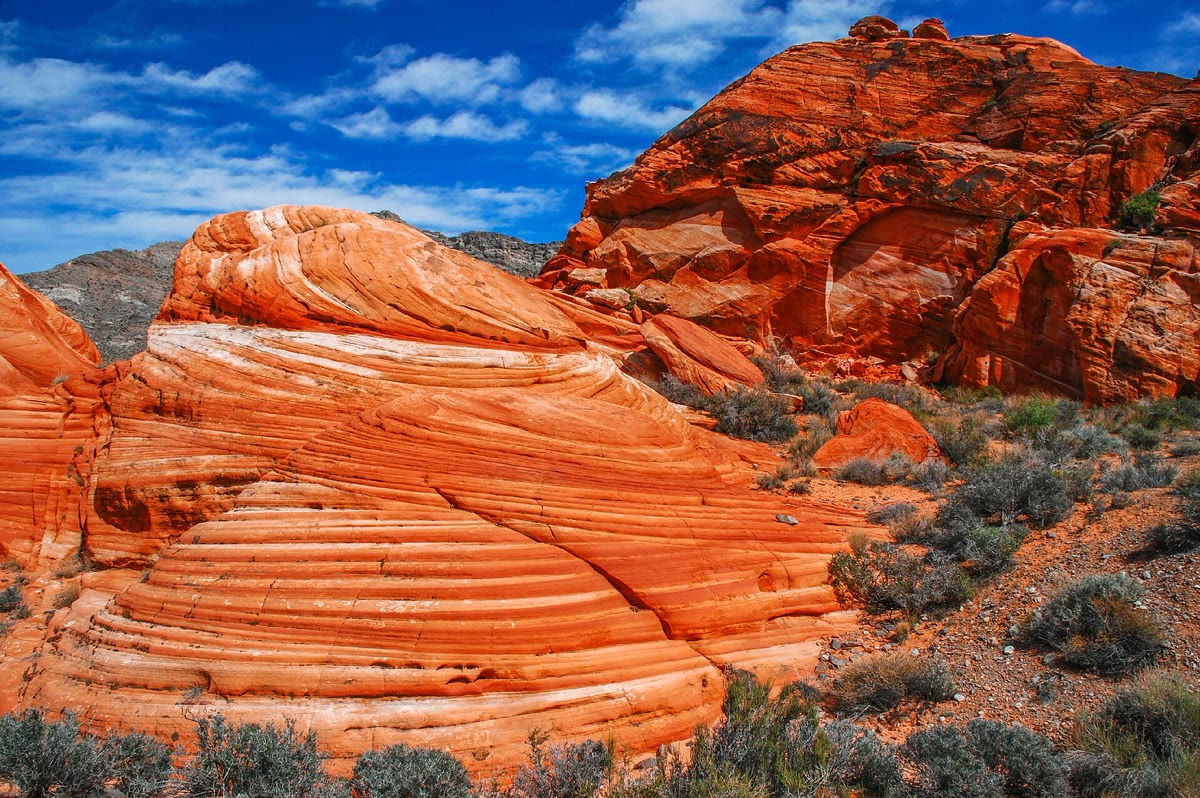
\includegraphics[height=3.6cm]{images/book3/b1-cross-bedding-aztec.jpg}};
\end{tikzpicture}

{\small Links: de geometrie van klimmende \omterm{def:b1:clastic-sediments:bedform}{bodemvormen} (schematisch, hoeken overdreven). De dalen bewegen zich langs rechte banen die onder de klimhoek $\theta$ hellen (dikke lijnen); tussen twee ervan blijven de onderste delen van de voorlagen behouden, in sets van dikte $T = L\sin\theta$. Rechts: \omterm{def:b1:clastic-sediments:cross-bedding}{kruislagen} in de Aztec-zandsteen, Muddy Mountains, Nevada: schuine sets van lamina's, elk bovenaan afgesneden door het erosievlak aan de basis van de volgende. Foto Chip Carroon, Bureau of Land Management, CC~BY-SA~2.0, via Wikimedia Commons.}
\label{fig:b1:clastic-sediments:climb}
\end{omfigure}
% ledger: southard:climb, commons:aztec-crossbed

\emph{Paleostromen.} De \omterm{def:b1:geological-maps:attitude}{hellingrichtingen} van \omterm{def:b1:clastic-sediments:cross-bedding}{kruislagen} die op een \omterm{def:b1:geological-maps:geological-map}{ontsluiting} zijn gemeten, verspreiden zich rond de gemiddelde richting van de stroming, omdat de lee-vlakken van \omterm{def:b1:clastic-sediments:bedform}{duinen} en \omterm{def:b1:clastic-sediments:bedform}{rimpels} gebogen zijn en de stromingen zelf zwerven. Hun gemiddelde wordt genomen als een vectorgemiddelde, niet als een rekenkundig gemiddelde, om de reden die in \cref{prop:b1:field-lab-methods-1:vector-mean} wordt getoond: \omterm{def:b1:spherical-astronomy:horizontal}{azimuten} zijn hoeken op een cirkel, en 350 en 010 middelen tot 000, niet tot 180.

\begin{proposition}[Gemiddelde van azimuten]\label{prop:b1:clastic-sediments:azimuths}
Laat $\alpha_1, \ldots, \alpha_N$ \omterm{def:b1:spherical-astronomy:horizontal}{azimuten} zijn, gemeten met de klok mee vanaf het noorden. Hun vectorgemiddelde $\bar\alpha$ en hun gemiddelde resultante-lengte $\bar R$ worden gegeven door
\[
  S = \sum_{i=1}^N \sin\alpha_i, \quad C = \sum_{i=1}^N \cos\alpha_i, \quad
  \bar\alpha = \operatorname{atan2}(S, C), \quad \bar R = \frac{\sqrt{S^2 + C^2}}{N},
\]
waarbij $\operatorname{atan2}(S, C)$ de hoek is waarvan sinus en cosinus evenredig zijn met $S$ en $C$, genomen tussen \ang{0} en \ang{360}. $\bar R$ ligt tussen 0 en 1 en is alleen 1 als alle \omterm{def:b1:spherical-astronomy:horizontal}{azimuten} gelijk zijn.
\end{proposition}

\begin{proof}
De eenheidsvector van \omterm{def:b1:spherical-astronomy:horizontal}{azimut} $\alpha$, met oost als eerste coördinaat en noord als tweede, is $(\sin\alpha, \cos\alpha)$. De som van de $N$ eenheidsvectoren is $(S, C)$, en haar richting, het vectorgemiddelde (\cref{def:b1:field-lab-methods-1:mean-orientation}), heeft de \omterm{def:b1:spherical-astronomy:horizontal}{azimut} waarvan sinus en cosinus $S/\sqrt{S^2+C^2}$ en $C/\sqrt{S^2+C^2}$ zijn. Door de driehoeksongelijkheid is de lengte van een som van $N$ eenheidsvectoren ten hoogste $N$, met gelijkheid alleen wanneer zij allemaal dezelfde kant op wijzen.
\end{proof}

\begin{method}[Paleostroom uit kruislagen]\label{met:b1:clastic-sediments:palaeocurrent}
\begin{enumerate}
  \item Meet op elke set de \omterm{def:b1:geological-maps:attitude}{hellingrichting} van de voorlagen, en kies vlakken die hun ware helling tonen (of meet \omterm{def:b1:geological-maps:attitude}{strijk} en helling).
  \item Meet de ligging van de hoofdlaagdeling; als zij meer dan een paar graden gekanteld is, draai dan elke voorlaag terug naar de horizontale om de \omterm{def:b1:geological-maps:attitude}{strijk} van de laagdeling (een rotatie die met de stereografische projectie van Boek~5 wordt gedaan).
  \item Bereken het vectorgemiddelde $\bar\alpha$ en $\bar R$ van de gecorrigeerde \omterm{def:b1:geological-maps:attitude}{hellingrichtingen} (\cref{prop:b1:clastic-sediments:azimuths}).
  \item Zet de metingen uit als een rozendiagram, een cirkelvormig histogram van \omterm{def:b1:spherical-astronomy:horizontal}{azimuten}, om te zien of zij één groep of twee vormen: getijstromingen die omkeren bouwen sets die in tegengestelde richtingen helen, in visgraatkruislagen, en één gemiddelde is dan zinloos.
\end{enumerate}
\end{method}
% ledger: og:sorting-environments

\emph{Andere structuren.} Verschillende andere structuren leggen de omstandigheden van afzetting en de rechtopstaande stand van de lagen vast. Een \omterm{def:b1:clastic-sediments:turbidite}{gegradeerde laag} wordt naar boven fijner, van grof aan de basis tot fijn aan de top, terwijl korrels uit een afnemende stroming bezinken, de grofste eerst (\cref{def:b1:clastic-sediments:turbidite}). Modderscheuren, veelhoeken van krimpscheuren die door de volgende laag worden gevuld, ontstaan waar modder aan de lucht droogt, zoals op getijvlakten en in uiterwaarden. Uitschuringen die de stroming in de modder eronder heeft gesneden, en die door het zand erboven worden gevuld, blijven bewaard als afgietsels op de basis van de zandsteenlaag, en hun vorm wijst de richting die de stroming nam.
% ledger: og:sorting-environments

\section{Facies, rivieren en delta's}\label{sec:b1:clastic-sediments:rivers-deltas}

Korrelgrootte, \omterm{def:b1:clastic-sediments:sorting}{sortering}, structuren, fossielen en samenstelling maken samen het karakter van een sedimentair gesteente, en geologen gebruiken één woord voor dat karakter.

\begin{definition}[Sedimentaire facies, afzettingsmilieu]\label{def:b1:clastic-sediments:facies}
Een \emph{sedimentaire facies}\index{sedimentaire facies} is een lichaam van sedimentair gesteente dat van andere wordt onderscheiden door zijn lithologie, korrelgrootte, sedimentaire structuren en fossielen, die alle de omstandigheden weerspiegelen waaronder het is gevormd. Het \emph{afzettingsmilieu}\index{afzettingsmilieu} is de plaats, met haar fysische, chemische en biologische omstandigheden, waarin een sediment wordt neergelegd: een rivierbedding, een uiterwaarde, een strand, de helling van een delta, de diepzeebodem.
\end{definition}
% ledger: og:sorting-environments

Een facies is een beschrijving, een milieu een interpretatie, en verschillende milieus kunnen dezelfde facies maken: gerimpeld zand wordt in rivieren, op getijvlakten en op de diepzeebodem afgezet. De interpretatie rust daarom op associaties van facies en op de volgorde waarin zij worden gestapeld, die de beweging van de milieus in de ruimte volgen: de algemene wetten van die stapeling, en de standaardmodellen van elk milieu, zijn het onderwerp van Boek~5. Dit hoofdstuk beschrijft de belangrijkste klastische milieus en de verticale opeenvolgingen die ze identificeren.

\emph{Vlechtende en meanderende rivieren.} Rivieren komen in twee hoofdstijlen voor. Een vlechtende rivier stroomt in vele geulen die zich splitsen en weer samenkomen rond banken van grind en zand; vlechtende rivieren voeren nabij hun bronnen grove vrachten, onder bergen of voor gletsjers, en hun afzettingen zijn lagen van grind en grof, kruisgelaagd zand, met weinig modder. Een meanderende rivier stroomt in één kronkelende geul. Het snelste water loopt langs de buitenkant van elke bocht, waar het de afslagoever uitschuurt; aan de binnenkant, waar het water het langzaamst is, wordt zand afgezet op de puntbank. De meander migreert zo zijwaarts, eroderend aan de ene zijde en opbouwend aan de andere; de uiterwaarde voorbij de oevers ontvangt alleen de modder van de overstromingen.
% ledger: og:rivers

De opeenvolging van de puntbank volgt uit de \omterm{def:b1:clastic-sediments:bedform}{bodemvormen}. Aan de voet van de bank, in het diepste en snelste water, laat de stroming de grofste korrels achter en bouwt zij \omterm{def:b1:clastic-sediments:bedform}{duinen}; hoger op de zachtglooiende bank wordt het water ondieper en langzamer, het zand fijner, en de \omterm{def:b1:clastic-sediments:bedform}{duinen} maken plaats voor \omterm{def:b1:clastic-sediments:bedform}{rimpels} (\cref{sec:b1:clastic-sediments:bedforms}); bovenaan gaat de bank over in de uiterwaarde. Naarmate de bocht migreert, beweegt elk van deze zones over die eronder, en een boring door de afzetting treft ze gestapeld aan: een naar boven fijner wordende opeenvolging van een erosievlak
tot modder, één voor elke passage van een geul, waarvan de dikte ongeveer de diepte is van de geul die haar maakte.

\emph{Delta's.} Waar een rivier een stilstaand water binnenkomt, spreidt en vertraagt haar stroming zich, en wordt haar vracht neergelegd: de grove vracht dicht bij de monding, de fijne verder weg. Een delta groeit vooruit, of progradeert, zolang de rivier meer sediment aanvoert dan golven en getij kunnen wegdragen. Wat golven en getij met de aanvoer doen, bepaalt haar vorm.

\begin{definition}[Door rivieren, golven en getij gedomineerde delta's]\label{def:b1:clastic-sediments:delta}
Een delta is \emph{door rivieren gedomineerd}\index{door rivieren gedomineerde delta} wanneer de aanvoer van de rivier de golven en het getij overweldigt, en haar distributaire geulen, ingesloten door hun eigen oeververhogingen, lange vingers van zand in de zee bouwen; zij is \emph{door golven gedomineerd}\index{door golven gedomineerde delta} wanneer golven het zand dat naar de monden is gebracht, verwerken tot stranden en strandwallen langs een gladde, gebogen kust; zij is \emph{door getij gedomineerd}\index{door getij gedomineerde delta} wanneer getijstromingen, die in en uit de monden stromen, haar zand vormen tot banken en ruggen evenwijdig aan de stroming, gescheiden door trechtervormige geulen.
\end{definition}
% ledger: og:deltas

\begin{omfigure}
\begin{tikzpicture}[font=\footnotesize, >={Stealth[length=4pt]}]
% meander in plan view (schematic) and the fining-upward log of a point bar
\begin{scope}[yscale=0.8]
  \fill[green!8] (-0.2,-0.4) rectangle (7.2,4.4);
  \draw[omSea!80!black, line width=9pt] plot[smooth, tension=0.7] coordinates {(0,3.6) (1.4,3.7) (2.6,2.8) (2.3,1.4) (3.2,0.5) (4.6,0.8) (5.0,2.2) (5.6,3.4) (7.0,3.5)};
  \draw[omSea!45, line width=7pt] plot[smooth, tension=0.7] coordinates {(0,3.6) (1.4,3.7) (2.6,2.8) (2.3,1.4) (3.2,0.5) (4.6,0.8) (5.0,2.2) (5.6,3.4) (7.0,3.5)};
  % point bars (inside of bends) with scroll lines
  \foreach \r in {0.25,0.45,0.65} {\draw[brown!60!black, densely dotted] (3.45,1.15) ++(200:\r) arc[start angle=200, end angle=340, radius=\r];}
  \fill[brown!25, opacity=0.8] (3.45,1.25) ellipse[x radius=0.55, y radius=0.35];
  \node[align=center] at (3.45,1.95) {puntbank\\ (afzetting)};
  \fill[brown!25, opacity=0.8] (1.75,2.75) ellipse[x radius=0.4, y radius=0.45];
  \node[align=center] at (1.3,1.95) {puntbank};
  \draw[red!60!black, thick] (2.9,0.2) .. controls (3.3,0.0) and (4.3,0.15) .. (4.85,0.6);
  \node[red!60!black, anchor=north] at (4.0,0.0) {afslagoever (erosie)};
  \draw[->, black!70] (5.9,3.0) -- (6.7,3.15) node[right] {stroming};
  \node[anchor=north west, black!60] at (5.2,1.3) {uiterwaarde};
  \node[font=\footnotesize] at (3.5,-0.85) {(a) een meander, in grondplan};
\end{scope}
\begin{scope}[xshift=9.2cm, yshift=-0.3cm, yscale=0.8]
  % log: x width = grain size; y = height
  \draw[lith shale] (0,3.6) rectangle (0.8,4.6);
  \draw[lith sandstone] (0,2.6) rectangle (1.2,3.6);
  \draw[lith sandstone] (0,0.6) rectangle (1.7,2.6);
  \draw[lith conglomerate] (0,0) rectangle (2.2,0.6);
  \draw[very thick, red!60!black] (0,0) -- (2.2,0);
  % cross-bed symbols
  \foreach \y in {0.9,1.5,2.1} {\draw[black!70] (0.3,\y) .. controls (0.6,\y+0.05) and (0.9,\y+0.25) .. (1.2,\y+0.4);}
  \foreach \x in {0.2,0.5,0.8} {\draw[black!70] (\x,3.0) -- ++(0.12,0.1) -- ++(0.12,-0.1);}
  \node[anchor=west, align=left] at (2.4,4.1) {uiterwaardemodder,\\ wortels, modderscheuren};
  \node[anchor=west, align=left] at (2.4,3.1) {fijn zand, rimpelkruislaminatie};
  \node[anchor=west, align=left] at (2.4,1.6) {middelgrof tot grof zand,\\ duinkruislagen};
  \node[anchor=west, align=left] at (2.4,0.3) {grindlaag op een\\ erosievlak};
  \draw[->] (-0.35,0) -- (-0.35,4.6) node[above] {omhoog};
  \draw[<->, black!60] (-0.7,0) -- node[above, rotate=90, font=\scriptsize] {geuldiepte} (-0.7,3.6);
  \node[font=\footnotesize] at (1.8,-0.5) {(b) opeenvolging van de puntbank};
\end{scope}
\end{tikzpicture}

{\small (a)~Een meanderende rivier (schematisch): de stroming erodeert de buitenoever van elke bocht en legt zand af op de puntbank binnenin; de gebogen schaallijnen zijn de opeenvolgende posities van de bank. (b)~De opeenvolging die een migrerende puntbank achterlaat, met de breedte van elke laag evenredig aan haar korrelgrootte (schematisch). Zij wordt naar boven fijner, en haar dikte legt de diepte van de geul vast.}
\label{fig:b1:clastic-sediments:point-bar}
\end{omfigure}
% ledger: og:rivers, southard:phase-diagram

De drie uiteinden zijn de hoekpunten van een driehoek waarin elke delta kan worden geplaatst door de relatieve sterkte van de drie processen. De vogelpootdelta van de Mississippi, met haar lange vingers in de Golf van Mexico (\cref{ch:b1:erosion-transport}), is de klassieke \omterm{def:b1:clastic-sediments:delta}{door rivieren gedomineerde delta}; de Nijl, met haar gladde boog van stranden, een door golven gedomineerde; de delta van de Ganges en de Brahmaputra, de grootste ter wereld, een door getij gedomineerde.
% ledger: og:deltas

\begin{omfigure}
\begin{tikzpicture}[font=\footnotesize]
% delta classification triangle (schematic) and the Lena delta from Landsat
\begin{scope}[yscale=0.82]
  \coordinate (R) at (2.6,4.5); \coordinate (W) at (0,0); \coordinate (T) at (5.2,0);
  \fill[omDef!8] (R) -- (W) -- (T) -- cycle;
  \draw[thick] (R) -- (W) -- (T) -- cycle;
  \node[above, align=center] at (R) {\textbf{door rivieren gedomineerd}\\ lange vingers, oeverwallen};
  \node[below, align=center] at (W) {\textbf{door golven gedomineerd}\\ strandwallen};
  \node[below, align=center] at (T) {\textbf{door getij gedomineerd}\\ zandbanken langs de stroming};
  \fill[omThm] (2.6,2.9) circle[radius=2pt] node[below=1pt] {Mississippi};
  \fill[omThm] (0.75,0.4) circle[radius=2pt] node[above right=0pt] {Nijl};
  \fill[omThm] (4.4,0.4) circle[radius=2pt] node[above left=0pt, align=right] {Ganges--\\ Brahmaputra};
\end{scope}
\node[anchor=south west, inner sep=0] at (7.2,-0.9) {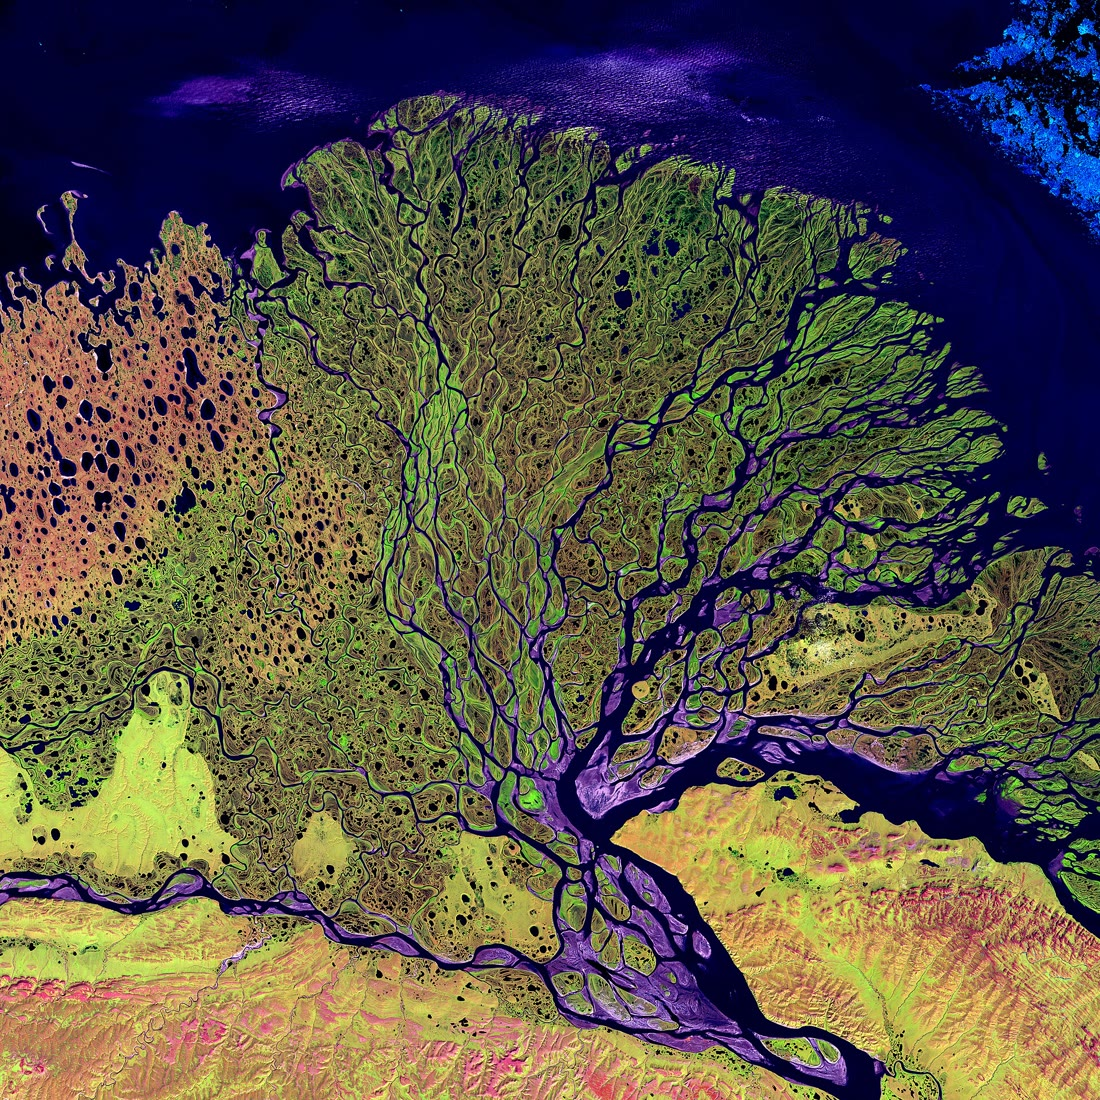
\includegraphics[height=5.2cm]{images/book3/b1-lena-delta.jpg}};
\end{tikzpicture}

{\small Links: de drie uiteinden van deltas, na het proces dat hen vormt (schematisch; de posities van de drie voorbeelden zijn indicatief). Rechts: de delta van de Lena, in Siberië, gebouwd in de Laptevzee (boven); de rivier komt van rechtsonder binnen en splitst zich in honderden distributaire geulen. Landsat~7-valse-kleurenbeeld van 27~februari 2000, U.S. Geological Survey, publiek domein, via Wikimedia Commons.}
\label{fig:b1:clastic-sediments:deltas}
\end{omfigure}
% ledger: og:deltas, commons:lena-delta

\emph{De opeenvolging die naar boven grover wordt.} Voor de monding van de rivier heeft de delta een zacht hellend front, het deltafront, dat zeewaarts overgaat in de prodelta, waar alleen modder uit suspensie bezinkt. Terwijl de delta progradeert, schuift elk van deze zones voort over de zone ervoor: een boring op de deltavlakte treft van onder naar boven de gelamineerde modders van de prodelta, dan wisselende silt en zand van het onderste deltafront, dan het kruisgelaagde zand van de monding-banken, boven afgesneden door de geulen van de deltavlakte. De opeenvolging wordt naar boven grover, het omgekeerde van een puntbank, en haar dikte is ongeveer de diepte van het water waarin de delta bouwde. Haar snelheid hangt samen met de geometrie van het deltafront.

\begin{proposition}[Progradatie en opstapeling]\label{prop:b1:clastic-sediments:progradation}
Laat een deltafront met constante helling $\alpha$ horizontaal voortschrijden met de snelheid $v$ zonder van vorm te veranderen, bij constant zeeniveau. Een vast punt onder het front ontvangt dan sediment met de verticale snelheid
\[
  a = v\,\tan\alpha,
\]
en de deltafrontopeenvolging van dikte $h$ hoopt zich daar op in de tijd $h/(v\tan\alpha)$.
\end{proposition}

\begin{proof}
In de tijd $\mathrm dt$ beweegt het front $v\,\mathrm dt$ vooruit. Op een vast punt onder het hellende oppervlak stijgt het oppervlak met het hoogteverschil tussen twee punten van het front op een horizontale afstand $v\,\mathrm dt$ van elkaar, dat is $v\,\mathrm dt\,\tan\alpha$, vandaar de snelheid. Het front passeert het punt terwijl het oppervlak met $h$ stijgt, wat de tijd $h/a$ kost.
\end{proof}

Deltafronten hellen zacht, dus is $\tan\alpha$ klein: het front van een delta schuift veel sneller op dan het sediment op een willekeurig punt eronder zich opstapelt (\cref{exo:b1:clastic-sediments:12}).

\begin{inthelab}[Een kern beschrijven]
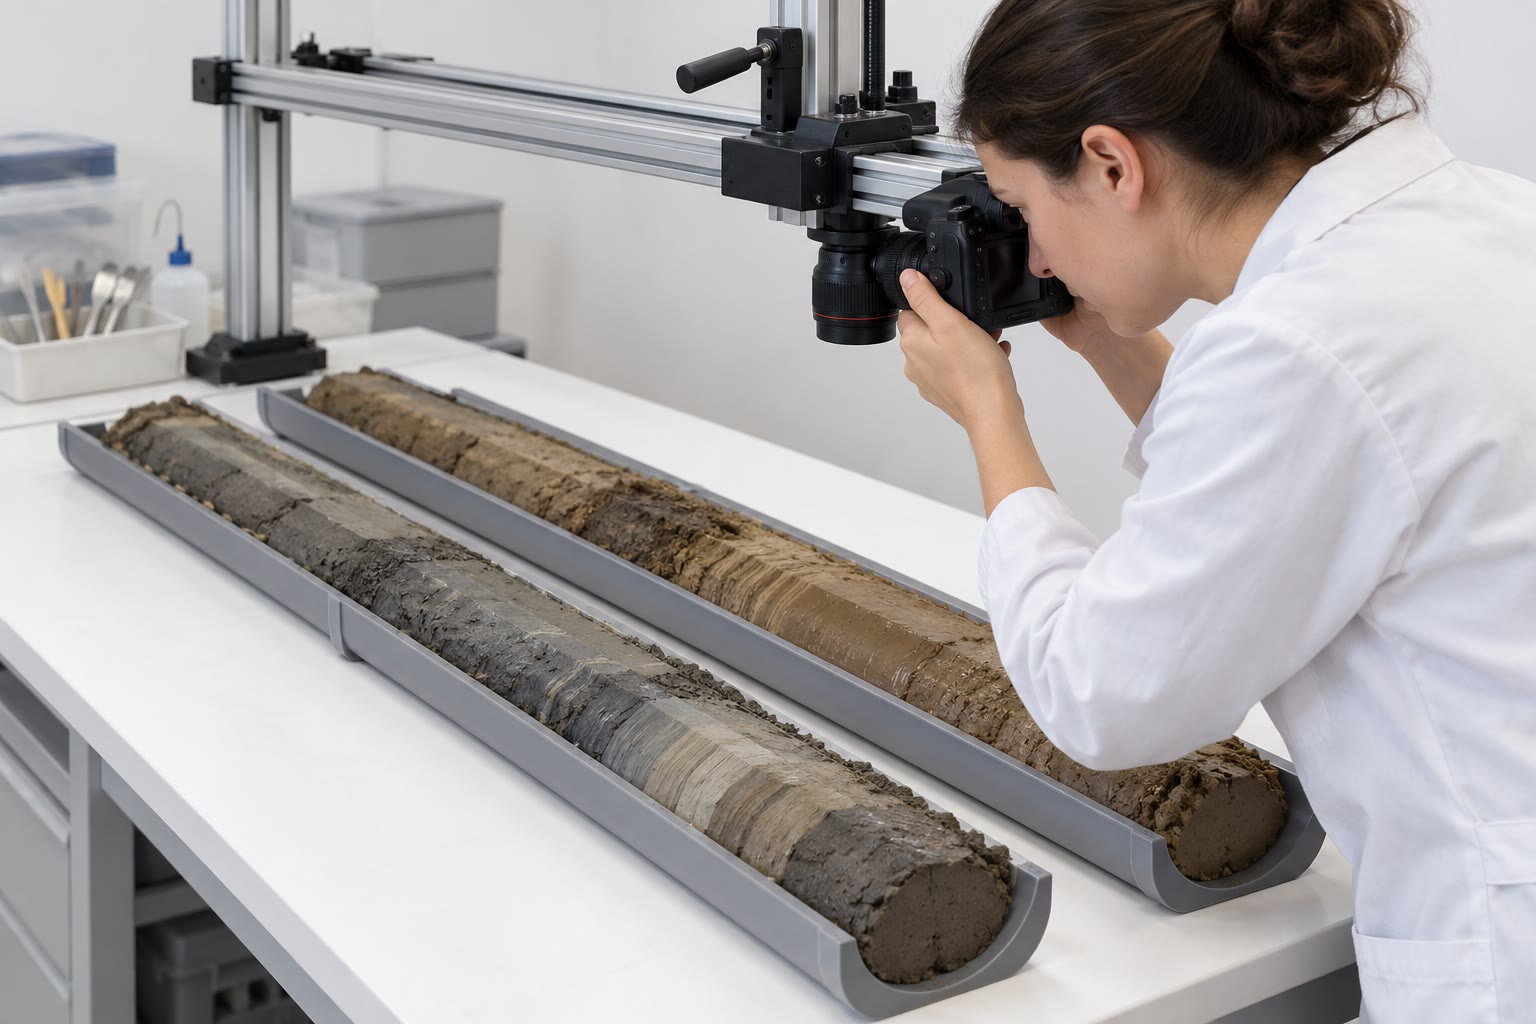
\includegraphics[width=0.3\linewidth]{images/book3/ai/b1-core-lab.jpg}\hfill
\begin{minipage}[b]{0.67\linewidth}
De cilinders sediment of gesteente die een boor naar boven brengt, worden in bakken in volgorde van diepte gelegd, in de lengte gespleten, en onder gelijkmatig licht gefotografeerd voordat zij drogen en van kleur veranderen. De sedimentoloog tekent dan een log van de kern, meter voor meter: de lithologie, de korrelgrootte van elke laag (de breedte van de kolom), de structuren (\omterm{def:b1:clastic-sediments:cross-bedding}{kruislagen}, laminatie, gradering, gangen), de \omterm{def:b1:geological-maps:geological-map}{contacten}, scherp of geleidelijk, de kleur en de fossielen. Er worden monsters genomen voor korrelgroottenanalyse en \omterm{def:b1:field-lab-methods-1:thin-section}{dunne slijpplaten}. Een kern is één smal venster: de richting van de \omterm{def:b1:clastic-sediments:cross-bedding}{kruislagen} gaat verloren tenzij de kern georiënteerd was, en de laterale uitbreiding van de lagen moet uit andere boringen komen.
\end{minipage}

\smallskip
{\small Een kern uitgelegd om te worden gefotografeerd in een sedimentlaboratorium (AI-illustratie).}
\end{inthelab}

\section{Kustlijn en continentaal plat}\label{sec:b1:clastic-sediments:shoreline}

Langs de kust tussen de delta's wordt het zand dat door de rivieren is aangevoerd gevormd door golven en getij. Een strand is zand dat door de swash wordt herwerkt, de dunne waterlaag die na elke brekende golf op en neer over het strand loopt: de korrels worden steeds opnieuw verplaatst, de fijne worden zeewaarts meegevoerd, en strandzanden behoren tot de best gesorteerde en meest afgeronde van alle sedimenten. Hun laminae, door de swash afgezet, hellen zacht zeewaarts. Op veel lage kusten vormt het zand barrière-eilanden, lange ruggen van strand en door de wind opgewaaide \omterm{def:b1:clastic-sediments:bedform}{duinen}, gescheiden van het vasteland door lagunes, die rustig en fijnkorrelig zijn en via getijdengeulen met de zee verbonden.

Waar het getij sterk is en de golven zwak, wordt de kust omzoomd door getijvlakten, twee keer per dag bedekt en onbedekt. Zij gaan van zand dicht bij de laagwaterlijn, waar de stromingen het sterkst zijn, naar modder dicht bij de hoogwaterlijn, waar het rustige water klei laat bezinken; hun afzettingen tonen de omkerende stroming in visgraatkruislagen, het drogen in modderscheuren, en de afwisseling van stroming en rustig water in dunne bedekkende modderlaagjes op gerimpeld zand.

Op het continentaal plat wordt de bodem door golven alleen tot een diepte geveegd die groeit met de grootte van de golven. Daarboven wordt zand uitgezeefd en verplaatst; daaronder bezinkt modder, behalve tijdens stormen, wanneer de grotere golven dieper reiken en lagen zand afzetten met de zachte golvende laminatie die heuvelige kruislaminatie heet. Een opeenvolging op het plat wisselt dus vaak af tussen modder van mooi weer en stormzanden, die dikker en grover worden naar de kust toe.
% ledger: og:sorting-environments, folk:maturity

\section{Diepzeeklastica}\label{sec:b1:clastic-sediments:deep-sea}

Zand en grind bereiken ook de bodems van de diepe oceanen, duizenden meters diep en honderden kilometers van het land, en ze worden daar gebracht door stromen die niemand volledig heeft gezien: dichte, met sediment beladen stromingen die de continentale helling afdalen onder het heldere water van de oceaan.

\begin{history}[Kabels op de zeebodem, 1929]
Op 18~november 1929 trof een aardbeving van \omterm{def:b1:earthquake-source:mw}{momentmagnitude} 7.2 de continentale helling ten zuiden van Newfoundland, langs de zuidrand van de Grand Banks. Een afschuiving van ongeveer \qty{200}{km^3} sediment bewoog zich op de helling, en een tsunami doodde 28 mensen aan de kust van Newfoundland. Twaalf telegraafkabels die over de zeebodem waren gelegd, braken, sommige op verschillende plaatsen. Die nabij het epicentrum braken meteen; de andere, verder naar het zuiden en dieper, braken de ene na de andere in de uren daarna, in volgorde van afstand naar beneden de helling. In 1952 verklaarden Bruce Heezen en Maurice Ewing, die de tijden van de breuken bestudeerden, ze: de afschuiving was veranderd in een \omterm{def:b1:clastic-sediments:turbidite}{troebelingsstroom} die de helling afliep en over de abyssale vlakte ging voor meer dan 480 mijl, en elke kabel brak toen zij passeerde. Uit de tijden en afstanden schatten zij haar snelheid op ongeveer 50 knopen op de bovenste continentale voet, waar de helling ongeveer \qty{0.5}{\percent} is, en nog 12 knopen bij de laatste kabel, ongeveer 400 mijl van haar oorsprong. Naarmate zij vertraagde, betoogden zij, moet zij een \omterm{def:b1:clastic-sediments:turbidite}{gegradeerde laag} over de vlakte hebben afgezet, naar boven steeds fijner.
\end{history}
% ledger: nrcan:grand-banks, he52:grand-banks

Vijftig knopen is \qty{25.7}{m.s^{-1}}, meer dan \qty{90}{km.h^{-1}}, de snelheid van een auto op een hoofdweg; 12 knopen is \qty{6.2}{m.s^{-1}}; en 480 mijl is ongeveer \qty{770}{km}. De breuken gaven ook de eerste gemeten snelheden van een stroming die alleen uit haar afzettingen en uit experimenten in tanks was afgeleid.
% ledger: he52:grand-banks

\begin{definition}[Troebelingsstroom, turbidiet, gegradeerde laag]\label{def:b1:clastic-sediments:turbidite}
Een \emph{troebelingsstroom}\index{troebelingsstroom} is een stroom water die door het sediment dat zij in suspensie houdt dichter wordt dan het water eromheen, en die onder dat water een helling afloopt, met haar korrels in suspensie gehouden door de turbulentie die haar eigen beweging maakt. Een \emph{turbidiet}\index{turbidiet} is de afzetting van een troebelingsstroom. Een \emph{gegradeerde laag}\index{gegradeerde laag} is een laag waarvan de korrelgrootte van haar basis naar haar top afneemt.
\end{definition}
% ledger: og:sorting-environments, he52:grand-banks

Een \omterm{def:b1:clastic-sediments:turbidite}{troebelingsstroom} drijft zichzelf aan: zij loopt omdat haar suspensie zwaar is, en zij houdt haar suspensie omdat zij loopt. Op een steile helling kan zij meer sediment van de bodem opnemen, dichter worden en versnellen; op de zachte helling van de abyssale vlakte vertraagt zij, laat haar vracht vallen en sterft zij uit.

\begin{proposition}[Snelheid van een troebelingsstroom]\label{prop:b1:clastic-sediments:turbidity}
Een \omterm{def:b1:clastic-sediments:turbidite}{troebelingsstroom} van dikte $h$ en dichtheid $\rho + \Delta\rho$ stroomt stationair een helling $S$ af onder water van dichtheid $\rho$. Als de weerstand van de bodem en van het water erboven $\tau = \rho\,C_f\,U^2$ per oppervlakte-eenheid is, waarbij $C_f$ een dimensieloze wrijvingscoëfficiënt is, is haar gemiddelde snelheid
\[
  U = \sqrt{\frac{\Delta\rho}{\rho}\,\frac{g\,h\,S}{C_f}} .
\]
\end{proposition}

\begin{proof}
De redenering is die van het diepte-helling-product (\cref{prop:b1:erosion-transport:depth-slope}), met het gewicht vervangen door het overgewicht. Een kolom van de stroom met eenheidsoppervlak weegt $(\rho +
\Delta\rho) g h$, en het water dat zij verplaatst $\rho g h$: in het omringende water trekt alleen het overschot $\Delta\rho\,g\,h$ haar de helling af, met de component $\Delta\rho\,g\,h\,S$ erlangs. In stationaire stroming houdt dit de weerstand $\rho C_f U^2$ in evenwicht, dus $U^2 = (\Delta\rho/\rho)\,g\,h\,S/C_f$.
\end{proof}

De weerstandswet $\tau = \rho C_f U^2$, kwadratisch in de snelheid, is die van turbulente stromingen in de hydraulica (de natuurkundeboeken), en $C_f$ wordt door experiment gevonden. De formule verwaarloost het water dat de stroom via haar bovenvlak in zichzelf mengt, wat haar verdunt en vertraagt. Zij toont de rol van de drie factoren: een stroom die tweemaal zo dik is, of tweemaal zo dicht, of op een tweemaal zo steile helling, loopt $\sqrt 2$ keer zo snel. Een suspensie die de fractie $c$ van haar volume als kwartskorrels houdt, heeft $\Delta\rho/\rho = 1.65\,c$ (\cref{sec:b1:erosion-transport:settling}), klein tenzij de stroming zeer geconcentreerd is; hier verschilt een \omterm{def:b1:clastic-sediments:turbidite}{troebelingsstroom} van een rivier, waarin het hele gewicht van het water, niet een klein overschot, de stroming drijft. Om met de \qty{50}{knopen} van 1929 te lopen op een helling van een halve procent, heeft een \omterm{def:b1:clastic-sediments:turbidite}{troebelingsstroom} een groot product van dikte en overdichtheid nodig (\cref{exo:b1:clastic-sediments:11}).

\emph{De reeks van Bouma.} In 1962 beschreef Arnold Bouma de inwendige orde van de zandsteenlagen van oude diepzeeopeenvolgingen in vijf divisies, van onder naar boven aangeduid. A: massief of gegradeerd zand, vaak op een erosieve basis; B: zand met evenwijdige laminatie; C: fijn zand met rimpelkruislaminatie, vaak gevouwen; D: gelamineerde silt die overgaat in modder; E: modder. De volgorde wordt gelezen als het verslag van één afnemende stroming die over een punt trekt: terwijl zij vertraagt, laat zij eerst haar grofste korrels in één keer vallen, bouwt dan een bovenste vlakke bodem, dan \omterm{def:b1:clastic-sediments:bedform}{rimpels}, en laat ten slotte de silt en klei bezinken. Volledige reeksen zijn zeldzaam: de bovenste divisies worden vaak door de volgende stroming weggeschuurd, en ver van de bron, waar de stroming zwak is, ontbreken de onderste.
% ledger: og:sorting-environments, shanmugam:bouma

\begin{omfigure}
\begin{tikzpicture}[font=\footnotesize]
% Bouma sequence: log (schematic) and a labelled photograph
\begin{scope}
  \draw[lith shale] (0,4.0) rectangle (0.7,4.8);
  \draw[lith shale] (0,3.3) rectangle (0.9,4.0);
  \draw[lith sandstone] (0,2.2) rectangle (1.3,3.3);
  \draw[lith sandstone] (0,1.2) rectangle (1.6,2.2);
  \draw[lith sandstone] (0,0) rectangle (2.0,1.2);
  \draw[very thick, red!60!black] (0,0) .. controls (0.6,-0.12) and (1.4,0.1) .. (2.0,0);
  \foreach \y in {1.4,1.6,1.8,2.0} {\draw[black!70] (0.1,\y) -- (1.5,\y);}
  \foreach \x in {0.15,0.5,0.85} {\draw[black!70] (\x,2.55) .. controls (\x+0.12,2.75) .. (\x+0.3,2.6);}
  \foreach \y in {3.45,3.6,3.75,3.9} {\draw[black!60] (0.1,\y) -- (0.8,\y);}
  \foreach \x/\y in {0.4/0.3, 0.9/0.5, 1.4/0.25, 0.6/0.8, 1.2/0.9} {\fill[black!60] (\x,\y) circle[radius=0.06];}
  \node[anchor=west] at (2.2,4.4) {E \quad modder};
  \node[anchor=west] at (2.2,3.65) {D \quad gelamineerde silt tot modder};
  \node[anchor=west] at (2.2,2.75) {C \quad rimpelkruislaminatie};
  \node[anchor=west] at (2.2,1.7) {B \quad evenwijdige laminatie};
  \node[anchor=west] at (2.2,0.6) {A \quad gegradeerd zand};
  \node[anchor=west, red!60!black] at (2.2,-0.15) {erosieve basis, zoolafdrukken};
  \draw[->] (-0.3,0) -- (-0.3,4.8) node[above] {omhoog};
\end{scope}
\node[anchor=south west, inner sep=0] at (6.9,-0.3) {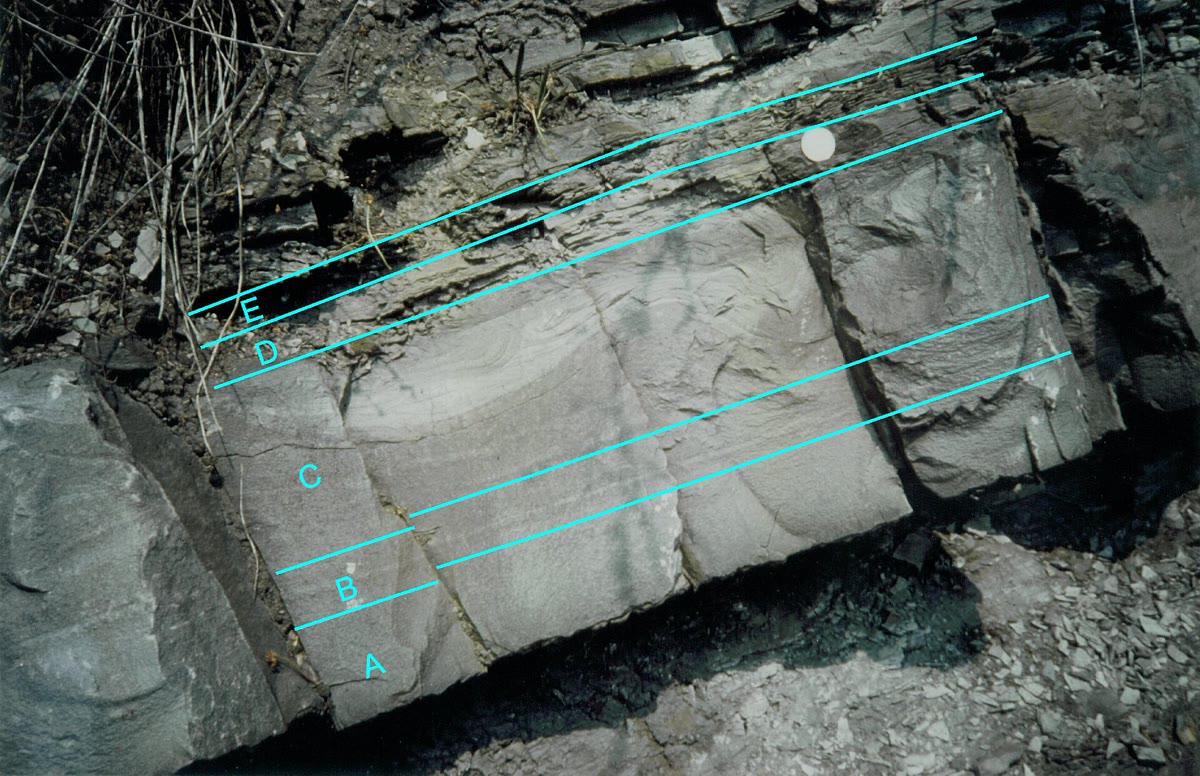
\includegraphics[height=5.2cm]{images/book3/b1-turbidite-bouma.jpg}};
\end{tikzpicture}

{\small Links: de vijf divisies van de reeks van Bouma, de breedte van elke evenredig aan haar korrelgrootte (schematisch). Rechts: een troebelingslaag van het Boven-Devoon bij Becke-Oese, Duitsland, met de divisies A tot E aangegeven door de fotograaf; de munt geeft de schaal. Foto Jo Weber, CC~BY-SA~3.0, via Wikimedia Commons.}
\label{fig:b1:clastic-sediments:bouma}
\end{omfigure}
% ledger: og:sorting-environments, shanmugam:bouma, commons:bouma-becke-oese

De reeks van Bouma werd het standaardmodel van de troebelingslaag, en duizenden oude diepzeezandsteenen zijn ermee geïnterpreteerd. De interpretatie is omstreden: stromingen langs de helling, diepe getijstromingen en interne golven bouwen ook gerimpelde en gelamineerde zanden, en sommige sedimentologen betogen dat veel lagen die als troebelingslagen worden gelezen, ook op de type-plaats, door andere stromen zijn afgezet. Weinig troebelingsstromingen zijn in de moderne oceaan waargenomen, terwijl oude troebelingslagen bij duizenden worden geteld.
% ledger: shanmugam:bouma

Niet alle diepzeeklastica zijn troebelingslagen. Contourstromen, de trage, diepe stromingen die de contouren van de continentale helling volgen, werken het sediment van de helling om tot gladde, langgerekte afzettingen, de contouritten. En ver van de continenten, waar noch troebelingsstromen noch contourstromen komen, ontvangt de zeebodem alleen wat uit het water erboven bezinkt: de schelpen van plankton en het fijnste door de wind aangevoerde stof, de pelagische sedimenten van het volgende hoofdstuk (\cref{ch:b1:chemical-biogenic-sediments}).
% ledger: og:sorting-environments

\section{Oefeningen}

\begin{exercise}[$\star$]\label{exo:b1:clastic-sediments:1}
Reken de diameters \qty{0.18}{mm}, \qty{0.75}{mm}, \qty{3}{mm}, \qty{0.012}{mm} en \qty{150}{mm} om naar phi-eenheden, tot op twee decimalen, en benoem de klasse van elk (\cref{tab:b1:clastic-sediments:classes}).
% ledger: folk:wentworth-classes
\end{exercise}

\begin{exercise}[$\star$]\label{exo:b1:clastic-sediments:2}
De cumulatieve kromme van een rivierzand geeft $\varphi_5 = 0.62$, $\varphi_{16} =
1.05$, $\varphi_{50} = 1.71$, $\varphi_{84} = 2.43$ en $\varphi_{95} = 2.98$. Bereken haar grafische gemiddelde, in phi-eenheden en in millimeter, en haar inclusieve grafische standaardafwijking, en benoem haar grootte en \omterm{def:b1:clastic-sediments:sorting}{sortering}.
% ledger: folk:graphic-measures, folk:sorting-classes
\end{exercise}

\begin{exercise}[$\star$]\label{exo:b1:clastic-sediments:3}
\omterm{def:b1:clastic-sediments:bedform}{Rimpels} van \qty{2}{cm} hoog migreren met \qty{1}{cm} per minuut over een bodem van kwartszand met porositeit \num{0.4}. Bereken met \cref{prop:b1:clastic-sediments:migration} het volume \omterm{def:b1:erosion-transport:load}{bodemvracht} per eenheid breedte, in \si{m^2.s^{-1}}, en de massa kwarts ($\qty{2650}{kg.m^{-3}}$) die per dag over een meter kam wordt vervoerd.
% ledger: hom:quartz
\end{exercise}

\begin{exercise}[$\star$]\label{exo:b1:clastic-sediments:4}
Een knoop is één nautische mijl, \qty{1852}{m}, per uur. (a)~Reken de snelheden van 50 en 12 knopen die voor de \omterm{def:b1:clastic-sediments:turbidite}{troebelingsstroom} van 1929 zijn geschat, om naar meter per seconde. (b)~Hoe lang doet een stroom van 12 knopen erover om \qty{100}{km} af te leggen? (c)~Reken 480 en 400 mijl om naar kilometer (één mijl is \qty{1.609}{km}).
% ledger: he52:grand-banks
\end{exercise}

\begin{exercise}[$\star\star$]\label{exo:b1:clastic-sediments:5}
(a)~Gebruik de percentielen van een normale verdeling die in het bewijs van \cref{prop:b1:clastic-sediments:normal} zijn gegeven, en bereken de grafische standaardafwijking
$(\varphi_{84} - \varphi_{16})/2$ en de schatting $(\varphi_{95} - \varphi_5)/3.3$ voor een normale verdeling met standaardafwijking $\sigma$. (b)~Leg uit waarom de twee voor een echt sediment oneens kunnen zijn. Welk soort sediment maakt ze het meest verschillend?
\end{exercise}

\begin{exercise}[$\star\star$]\label{exo:b1:clastic-sediments:6}
Een afzetting van klimmende \omterm{def:b1:clastic-sediments:bedform}{rimpels} toont sets van \qty{1.5}{cm} dik, gemeten loodrecht op hun grenzen, gemaakt door \omterm{def:b1:clastic-sediments:bedform}{rimpels} op \qty{15}{cm} van elkaar. (a)~Bereken de klimhoek. (b)~Als de \omterm{def:b1:clastic-sediments:bedform}{rimpels} met \qty{0.5}{cm} per minuut bewogen, met welke snelheid werd de bodem opgehoogd, in centimeter per uur? (c)~Leg uit wat zo'n snelheid over de stroming zegt.
% ledger: southard:climb
\end{exercise}

\begin{exercise}[$\star\star$]\label{exo:b1:clastic-sediments:7}
Zes \omterm{def:b1:geological-maps:attitude}{hellingrichtingen} van \omterm{def:b1:clastic-sediments:cross-bedding}{kruislagen}, al gecorrigeerd voor de kanteling van de lagen, lezen 350, 020, 005, 340, 015 en 030. (a)~Bereken hun rekenkundig gemiddelde. (b)~Bereken hun vectorgemiddelde en $\bar R$. (c)~Verklaar het verschil.
\end{exercise}

\begin{exercise}[$\star\star$]\label{exo:b1:clastic-sediments:8}
Drie zandstenen worden onder de \omterm{def:b1:field-lab-methods-1:thin-section}{dunne slijpplaat} onderzocht. A heeft \qty{12}{\percent} kleimatrix en hoekige korrels van kwarts, \omterm{def:b1:rock-forming-minerals:groups}{veldspaat} en gesteentefragmenten. B heeft \qty{2}{\percent} klei, $\sigma_I = 0.40\,\varphi$ en kwartskorrels met een afrondingsgraad \num{2.2} op de schaal van Folk. C heeft geen klei, $\sigma_I =
0.30\,\varphi$, kwartskorrels met een afrondingsgraad \num{3.6}, en \qty{98}{\percent} kwarts. Benoem de \omterm{def:b1:clastic-sediments:maturity}{textuurrijpheid} van elk, en stel voor elk een \omterm{def:b1:clastic-sediments:facies}{afzettingsmilieu} voor.
% ledger: folk:maturity
\end{exercise}

\begin{exercise}[$\star\star$]\label{exo:b1:clastic-sediments:9}
(a)~Bereken het Froude-getal van een stroming van \qty{0.3}{m} diep bij \qty{1.5}{m.s^{-1}}, en van een rivier van \qty{2}{m} diep bij \qty{1.0}{m.s^{-1}} ($g
= \qty{9.81}{m.s^{-2}}$). (b)~Bij welke diepte zou een stroming van \qty{1.5}{m.s^{-1}} een Froude-getal van 1 bereiken, en welke snelheid zou de rivier van \qty{2}{m} diep nodig hebben? (c)~Leg uit waarom antiduinen veel voorkomen in lagen water die van een strand af lopen, en zeldzaam zijn in grote rivieren.
% ledger: southard:ripples-dunes
\end{exercise}

\begin{exercise}[$\star\star\star$]\label{exo:b1:clastic-sediments:10}
Een zeefanalyse van een zand geeft, in hele-phi-klassen van $-1$ tot
$5\,\varphi$: 2, 8, 30, 40, 15 en 5 gewichtspercentage. (a)~Bereken met de methode van de momenten het gemiddelde en de standaardafwijking in phi-eenheden, en benoem de \omterm{def:b1:clastic-sediments:sorting}{sortering}. (b)~Bouw de cumulatieve kromme, lees $\varphi_5$, $\varphi_{16}$, $\varphi_{50}$, $\varphi_{84}$ en $\varphi_{95}$ af door lineaire interpolatie, en bereken $M_z$ en $\sigma_I$. (c)~Vergelijk.
% ledger: folk:graphic-measures, folk:sorting-classes
\end{exercise}

\begin{exercise}[$\star\star\star$]\label{exo:b1:clastic-sediments:11}
Neem $C_f = 0.003$ in \cref{prop:b1:clastic-sediments:turbidity}. (a)~Een \omterm{def:b1:clastic-sediments:turbidite}{troebelingsstroom} van \qty{50}{m} dik, met een overdichtheid van \qty{2}{\percent}, loopt een helling van \num{0.005} af: bereken haar snelheid, in meter per seconde en in knopen. (b)~Welk product van dikte en relatieve overdichtheid zou de 50 knopen van 1929 op dezelfde helling geven? (c)~Dezelfde stroming als in (a) bereikt een helling van \num{0.001}: bereken haar nieuwe snelheid, als er verder niets verandert. Wat gebeurt er met haar vracht?
% ledger: he52:grand-banks
\end{exercise}

\begin{exercise}[$\star\star\star$]\label{exo:b1:clastic-sediments:12}
Een rivier levert elk jaar \qty{50}{Mt} sediment aan haar delta, waarvan \qty{70}{\percent} wordt afgezet op een deltafront van \qty{100}{km} breed dat in water van \qty{30}{m} diep bouwt. Het afzetsel heeft een volumieke dichtheid van \qty{2000}{kg.m^{-3}}. (a)~Welk volume voegt het elk jaar toe? (b)~Als dit volume de hele waterdiepte langs de breedte van het front vult, hoe snel schuift het front vooruit? (c)~Met een helling van het deltafront van \ang{0.5}, met welke snelheid hoopt sediment zich op een vast punt onder het front op, en in hoeveel jaar vormt zich daar de naar boven grover wordende opeenvolging?
\end{exercise}

\section{Probleem: een kern uit een delta lezen}

\begin{problem}[{Weekendprobleem --- een boring door een oude delta, van de korrelgroottes tot de richting van haar rivieren}]
\label{pb:b1:clastic-sediments:1}
% values: calc/ch21.py; the borehole, its beds, ages and readings are invented
Een boring snijdt \qty{24}{m} zandsteen en modder door die door een oude delta
zijn afgezet. De geoloog beschrijft vier eenheden, van onder naar boven, en
analyseert van elk een monster.

\smallskip
\begin{center}\small
\begin{tabular}{@{}llccccc@{}}
\hline
eenheid (diepte vanaf de basis) & beschrijving & $\varphi_5$ & $\varphi_{16}$ & $\varphi_{50}$ & $\varphi_{84}$ & $\varphi_{95}$ \\
\hline
1 (0--8 m) & gelamineerde grijze modder & 4.2 & 5.0 & 6.6 & 8.4 & 9.6 \\
2 (8--16 m) & afwisselend siltsteen en zandsteen & 1.9 & 2.4 & 3.4 & 4.6 & 5.5 \\
3 (16--21 m) & kruisgelaagde zandsteen & 0.9 & 1.25 & 1.8 & 2.35 & 2.7 \\
4 (21--24 m) & grindrijke zandsteen, erosieve basis & $-1.8$ & $-0.8$ & 0.9 & 2.1 & 2.9 \\
\hline
\end{tabular}
\end{center}

\medskip
\noindent\textbf{Deel I --- De korrelgroottes.}
\begin{enumerate}
  \item Bereken het grafische gemiddelde $M_z$ van elke eenheid, in phi-eenheden
        en in millimeter.
  \item Bereken de inclusieve grafische standaardafwijking $\sigma_I$ van elke
        eenheid.
  \item Benoem de korrelgrootteklasse van het gemiddelde en de \omterm{def:b1:clastic-sediments:sorting}{sortering} van
        elke eenheid.
  \item Welke eenheid is het best gesorteerd? Waarom zou een mondingsbank beter
        gesorteerd zijn dan de modders van de prodelta?
  \item Interpoleer lineair tussen $\varphi_{50}$ en $\varphi_{84}$ en schat het
        percentage kleideeltjes (fijner dan $8\,\varphi$) in eenheid~1. Wat zegt
        dit over de stromingen waar zij werd afgezet?
  \item Waarom is de cumulatieve curve van eenheid~4 zo breed uitgespreid,
        hoewel het een geulzand is?
\end{enumerate}

\medskip
\noindent\textbf{Deel II --- De opeenvolging.}
\begin{enumerate}[resume]
  \item Beschrijf hoe de \omterm{def:b1:clastic-sediments:sorting}{gemiddelde korrelgrootte} verandert van eenheid~1 tot
        eenheid~3. Is de opeenvolging naar boven fijner of grover wordend?
  \item Interpreteer de eenheden 1, 2 en 3 als delen van een delta. Welke zone
        van de delta lag op de plaats van de boring toen elk werd afgezet?
  \item Wat laat de stapeling van de drie eenheden zien over de beweging van de
        delta?
  \item Minstens tot welke waterdiepte bouwde de delta uit, en waarom?
  \item Eenheid~4 heeft een erosieve basis en is grover dan eenheid~3. Interpreteer
        haar.
  \item Zou een puntbank dezelfde opeenvolging geven? Leg uit.
\end{enumerate}

\medskip
\noindent\textbf{Deel III --- Hoe snel rukte de delta op?}
Twee dunne lagen vulkanische as, aan de basis van eenheid~1 en aan de top van
eenheid~2, zijn gedateerd; ze liggen \num{4000}~jaar uit elkaar.
\begin{enumerate}[resume]
  \item Bereken de gemiddelde accumulatiesnelheid tussen de twee assen, in
        millimeter per jaar.
  \item Het deltafront hellde \ang{0.5}. Bereken met
        \cref{prop:b1:clastic-sediments:progradation} de snelheid waarmee het
        oprukte, in meter per jaar.
  \item Hoe ver rukte het front op in de \num{4000}~jaar?
  \item Hoe lang hebben de 21 meter van de eenheden 1 tot 3 er bij dit tempo over
        gedaan om zich ter plaatse op te hopen?
  \item Waarom is de accumulatiesnelheid in een delta niet overal op hetzelfde
        moment dezelfde?
\end{enumerate}

\medskip
\noindent\textbf{Deel IV --- Waar stroomden de rivieren?}
Op de kruisgelaagde zandsteen van eenheid~3, in een nabije \omterm{def:b1:geological-maps:geological-map}{ontsluiting} waar de
lagen horizontaal liggen, worden twaalf \omterm{def:b1:geological-maps:attitude}{hellingsrichtingen} van de foresets
gemeten: 352, 010, 025, 004, 338, 017, 031, 359, 012, 046, 006 en 344.
\begin{enumerate}[resume]
  \item Bereken het rekenkundig gemiddelde van de twaalf metingen. Heeft het zin?
  \item Bereken de sommen $S$ en $C$ van \cref{prop:b1:clastic-sediments:azimuths}.
  \item Bereken de gemiddelde resultantelengte $\bar R$. Zijn de metingen
        consistent?
  \item In welke algemene richting bouwde de delta, en waar lag het land?
  \item Waarom moeten de \omterm{def:b1:geological-maps:attitude}{hellingsrichtingen} worden geroteerd wanneer de lagen
        gekanteld zijn, en om welke as?
  \item Zou een getijdestroom deze \omterm{def:b1:clastic-sediments:cross-bedding}{kruislagen} hebben kunnen vormen? Hoe zou haar
        rozendiagram eruitzien?
  \item Wat is, op de graad nauwkeurig, de gemiddelde \omterm{def:b1:spherical-astronomy:horizontal}{paleostroom-azimut} van de
        kruisgelaagde zandsteen van eenheid~3?
\end{enumerate}
\end{problem}
